%------------------------------------------------------------------------------
%------------------------------------------------------------------------------
\newday{20180520}\label{20180520}

\newentry[Arrival and Setup]{0800 Arrival and Setup}
\FloatBarrier{}

Arrived at Damon Gunther's house for an introduction to beer brewing.  Damon already had his equipment setup (Figure~\ref{fig:setup}), in the driveway, and tools and ingredients laid out on a folding table (Figure~\ref{fig:tools}), inside the garage.  The end goal of this process is a homebrew clone of the Widmer Brothers Brewing Company Snowplow Milk Stout.

\begin{figure}[H]
\begin{minipage}{0.48\textwidth}
  \centering
  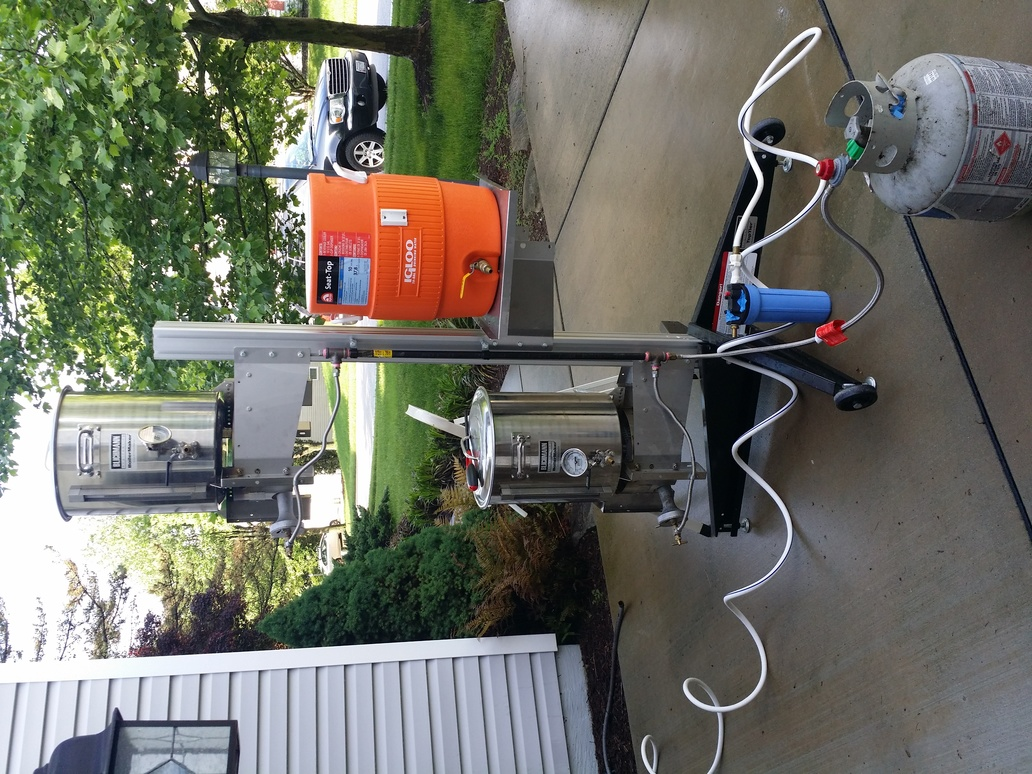
\includegraphics[angle=270,origin=c,width=\textwidth]{IMG_20180520_083244_reduced}
  \caption{Gravity feed brewing setup}\label{fig:setup}
\end{minipage}\hfill
\begin{minipage}{0.48\textwidth}
  \centering
  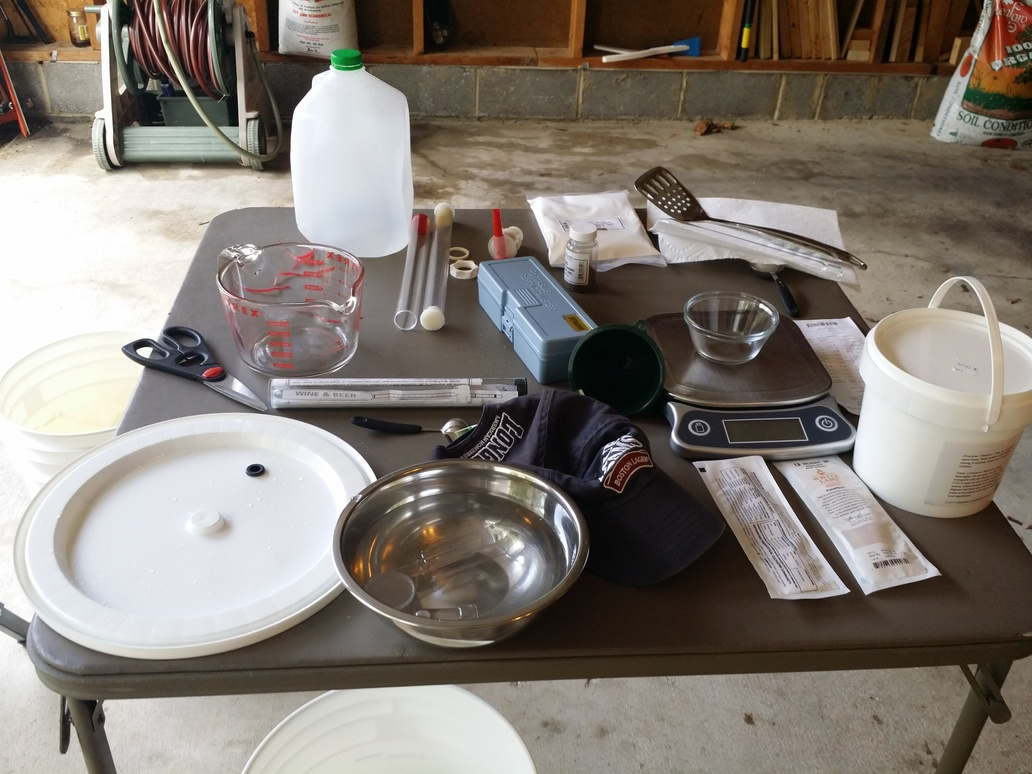
\includegraphics[width=\textwidth]{IMG_20180520_092957_reduced}
  \caption{Tools}\label{fig:tools}
\end{minipage}
\end{figure}

\FloatBarrier{}
\clearpage
%------------------------------------------------------------------------------
\newentry[Boil Filtered Water]{0830 Boil Filtered Water}\FloatBarrier{}

The top pot in Figure~\ref{fig:setup} is used to boil the \gls{strike water}, and also provides the heated \gls{sparge water} later in the process.  The \gls{strike water} must be heated to \SI{158} - \SI{173}\degree{}F.  When the strike water infuses with the grains to form the mash, the temperature will drop.  The ideal temperature range for the mash is \SI{148} - \SI{158}\degree{}F.  The temperature guage in Figure~\ref{fig:temp} is used to ensure the correct temperature of the water.

\begin{figure}[H]
  \centering
  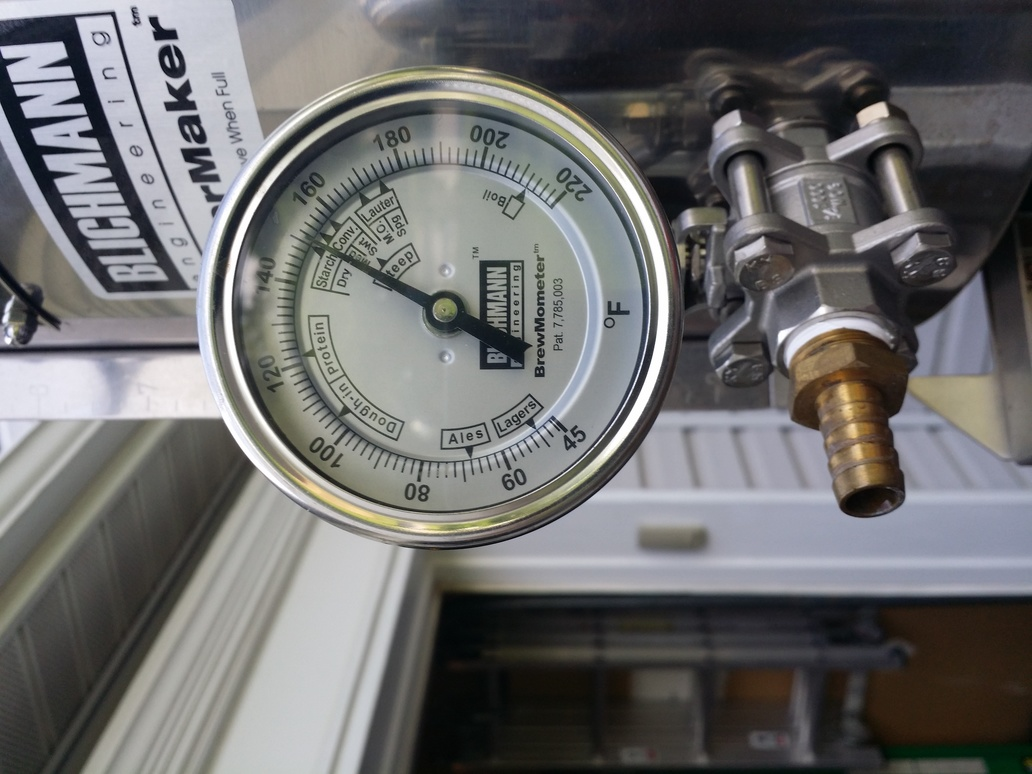
\includegraphics[angle=270,origin=c,width=0.5\textwidth]{IMG_20180520_083252_reduced}
  \caption{Temperature Guage}\label{fig:temp}
\end{figure}

\FloatBarrier{}
\clearpage
%------------------------------------------------------------------------------
\newentry[Mash In]{0845 Mash In}\FloatBarrier{}

Heated water goes in mash tun, also called the lautering tun.  All grains in the ingredients list \cref{subfig:flakedoats,subfig:tworow,subfig:crystalsixty,subfig:carapils,subfig:wheat,subfig:roastedbarley,subfig:black}, are stirred into the hot water in the lautering tun with the large stirring spoon. Check temperature in igloo. Desired temperatures will vary by recipie.  Start the timer for one hour, and start heating more water.

\begin{figure}[H]
\centering
\begin{subfigure}[b]{.245\textwidth}
  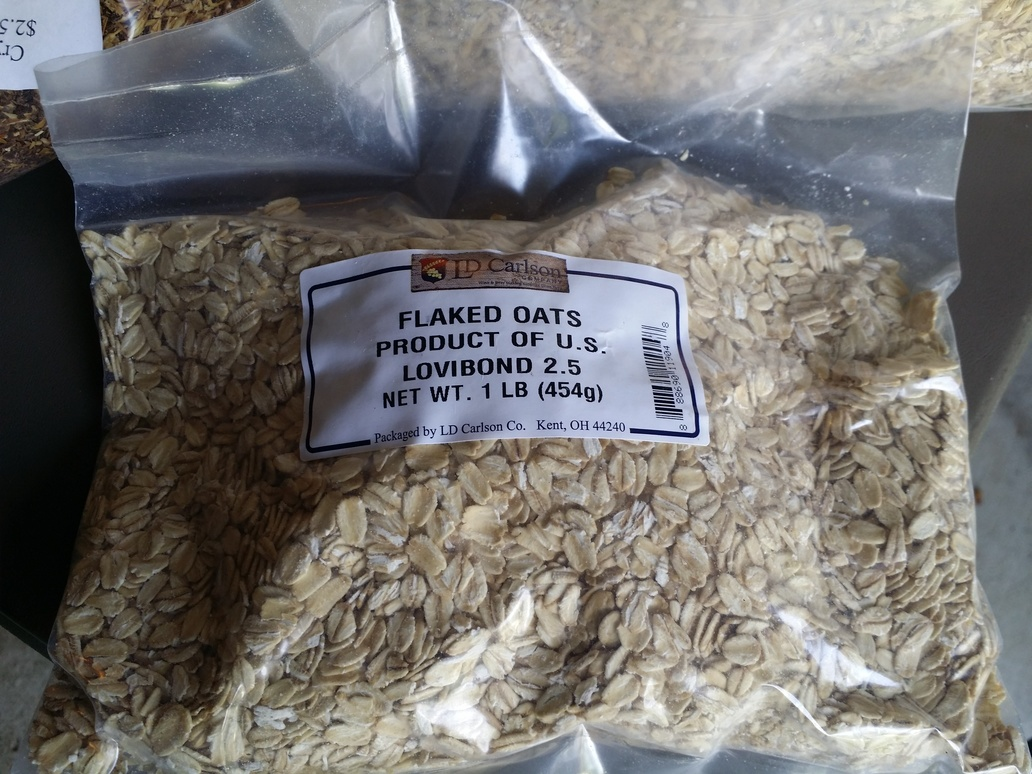
\includegraphics[width=\textwidth]{IMG_20180520_083053_reduced}
  \caption{Flaked Oats}\label{subfig:flakedoats}
\end{subfigure}
\begin{subfigure}[b]{.245\textwidth}
  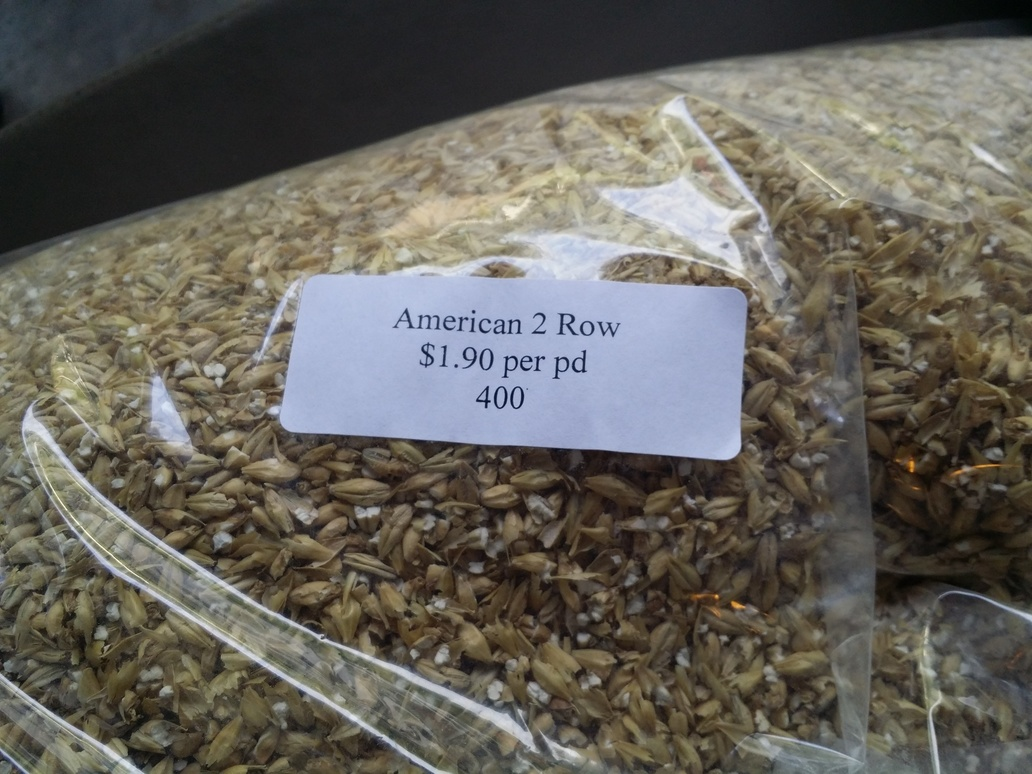
\includegraphics[width=\textwidth]{IMG_20180520_083103_reduced}
  \caption{American 2 Row}\label{subfig:tworow}
\end{subfigure}
\begin{subfigure}[b]{.245\textwidth}
  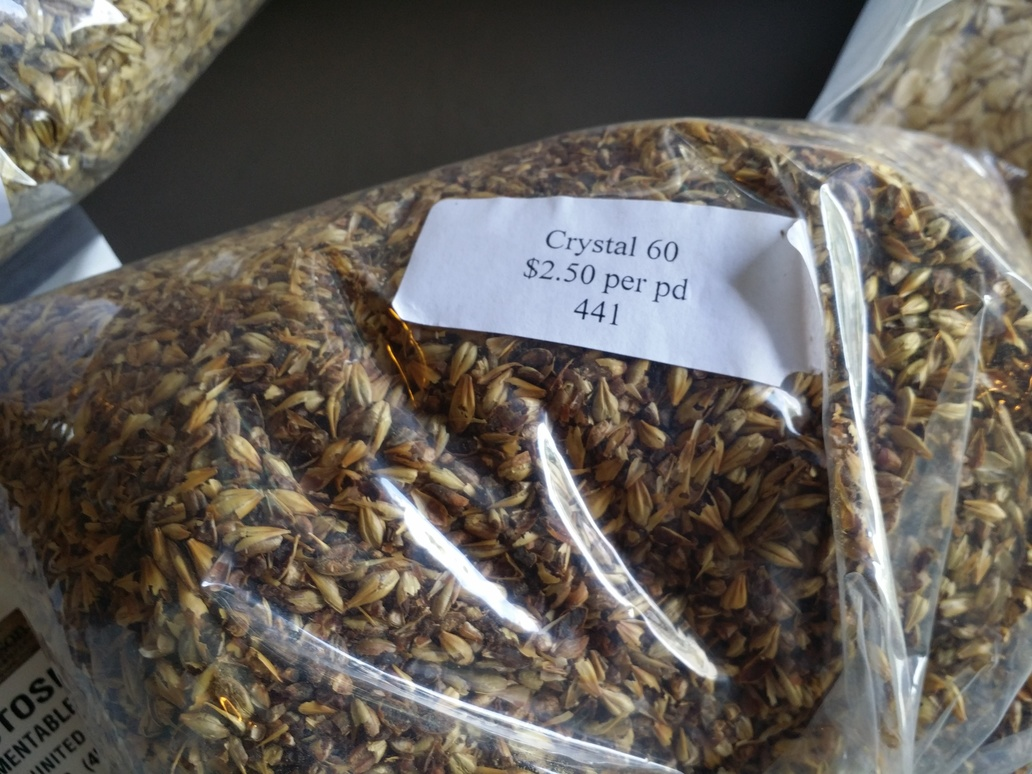
\includegraphics[width=\textwidth]{IMG_20180520_083110_reduced}
  \caption{Crystal 60}\label{subfig:crystalsixty}
\end{subfigure}
\begin{subfigure}[b]{.245\textwidth}
  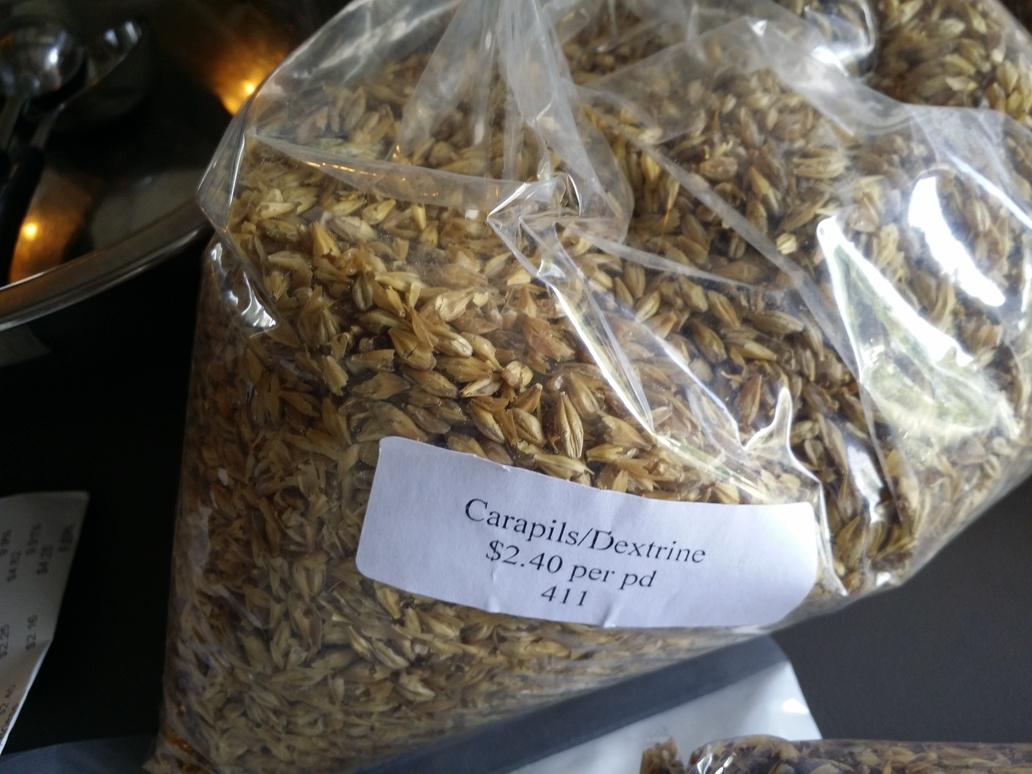
\includegraphics[width=\textwidth]{IMG_20180520_083114_reduced}
  \caption{Carapils/Dextrine}\label{subfig:carapils}
\end{subfigure}

\begin{subfigure}[b]{.245\textwidth}
  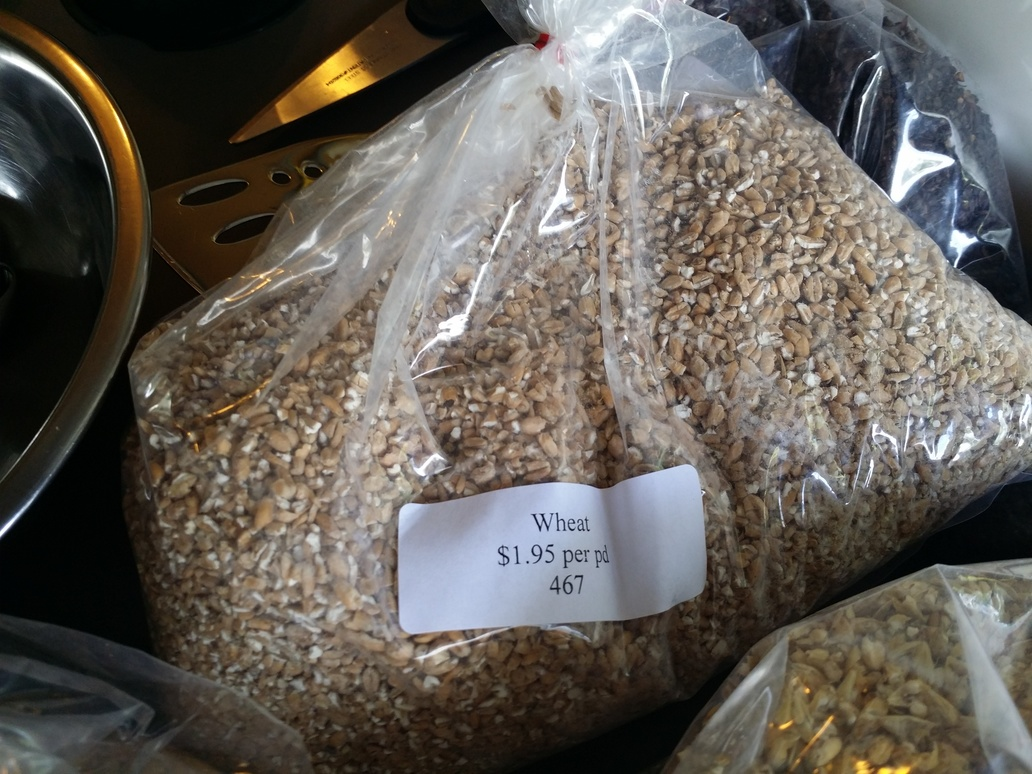
\includegraphics[width=\textwidth]{IMG_20180520_083120_reduced}
  \caption{Wheat}\label{subfig:wheat}
\end{subfigure}
\begin{subfigure}[b]{.245\textwidth}
  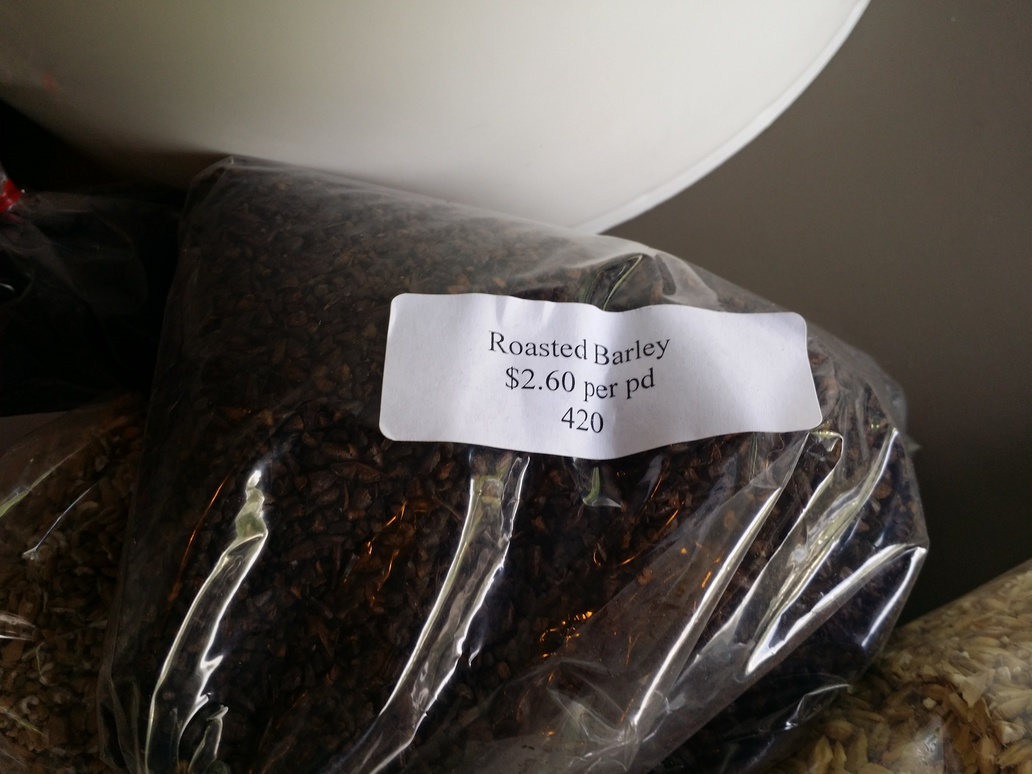
\includegraphics[width=\textwidth]{IMG_20180520_083130_reduced}
  \caption{Roasted Barley}\label{subfig:roastedbarley}
\end{subfigure}
\begin{subfigure}[b]{.245\textwidth}
  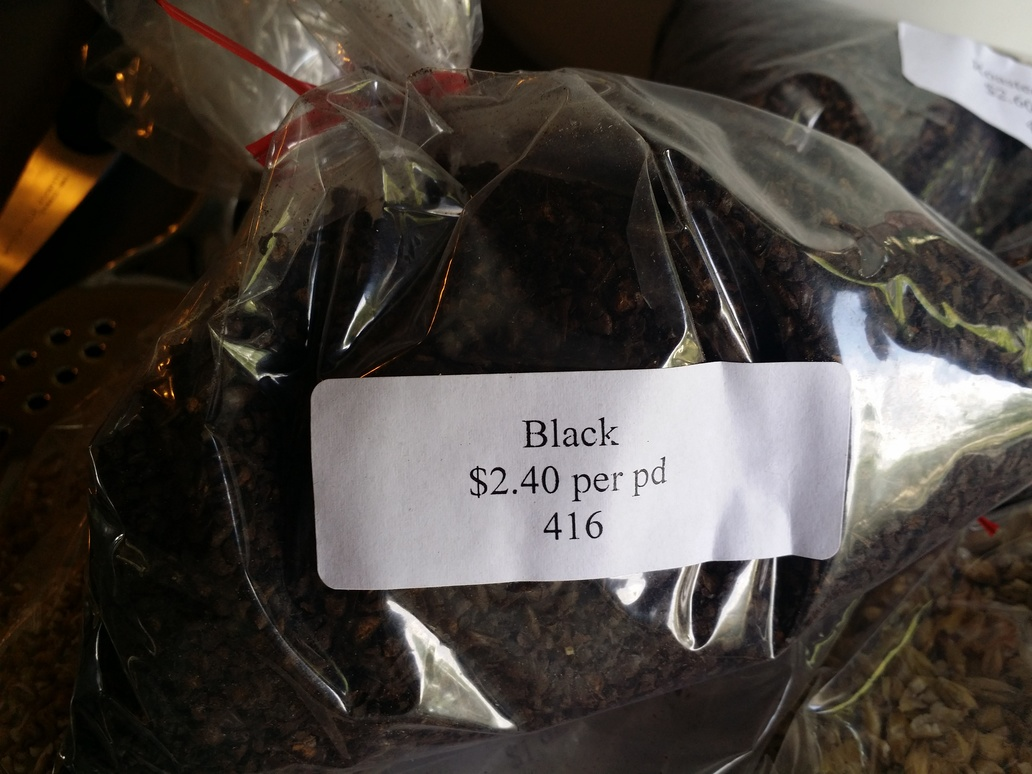
\includegraphics[width=\textwidth]{IMG_20180520_083135_reduced}
  \caption{Black}\label{subfig:black}
\end{subfigure}

\begin{subfigure}[b]{.245\textwidth}
  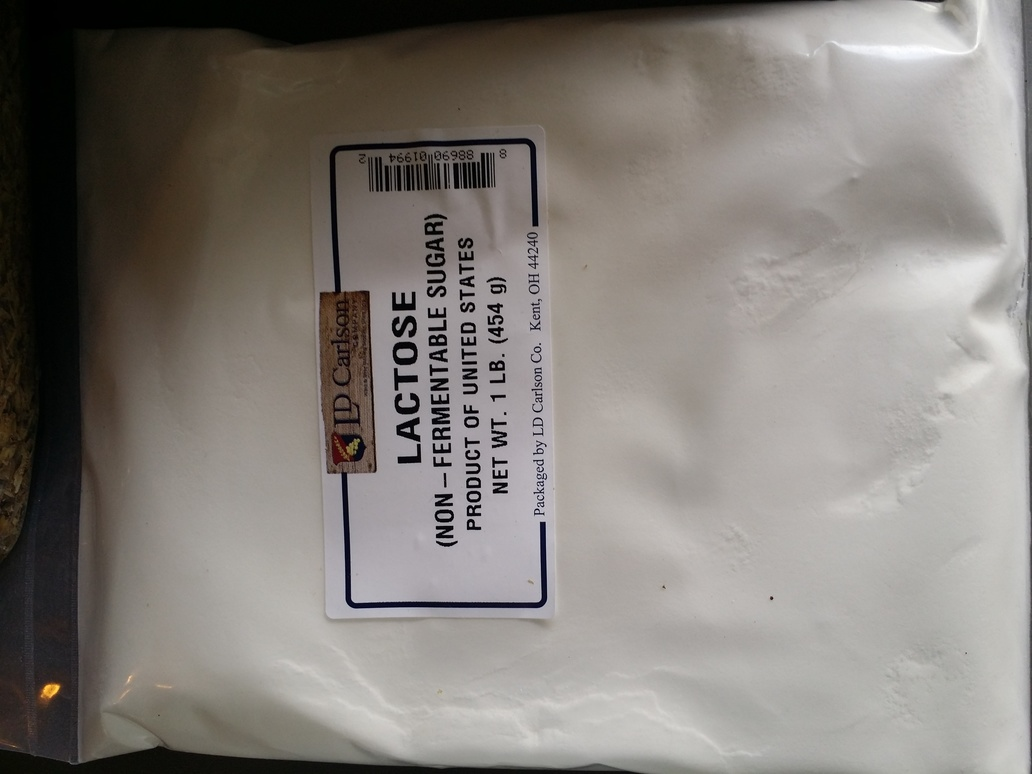
\includegraphics[angle=270,origin=c,width=\textwidth]{IMG_20180520_083204_reduced}
  \caption{Lactose}\label{subfig:lactose}
\end{subfigure}
\begin{subfigure}[b]{.245\textwidth}
  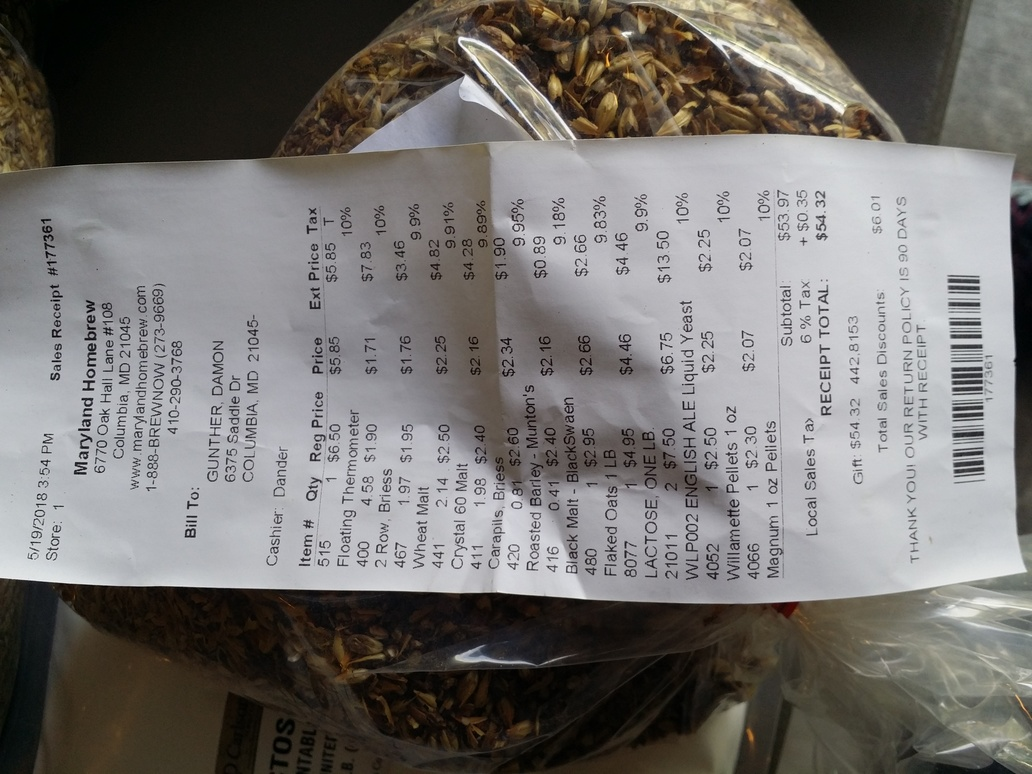
\includegraphics[angle=270,origin=c,width=\textwidth]{IMG_20180520_083145_reduced}
  \caption{Reciept}\label{subfig:receipt}
\end{subfigure}
\caption{Ingredients}\label{subfig:ingredients}
\end{figure}

\begin{figure}[H]
  \centering
  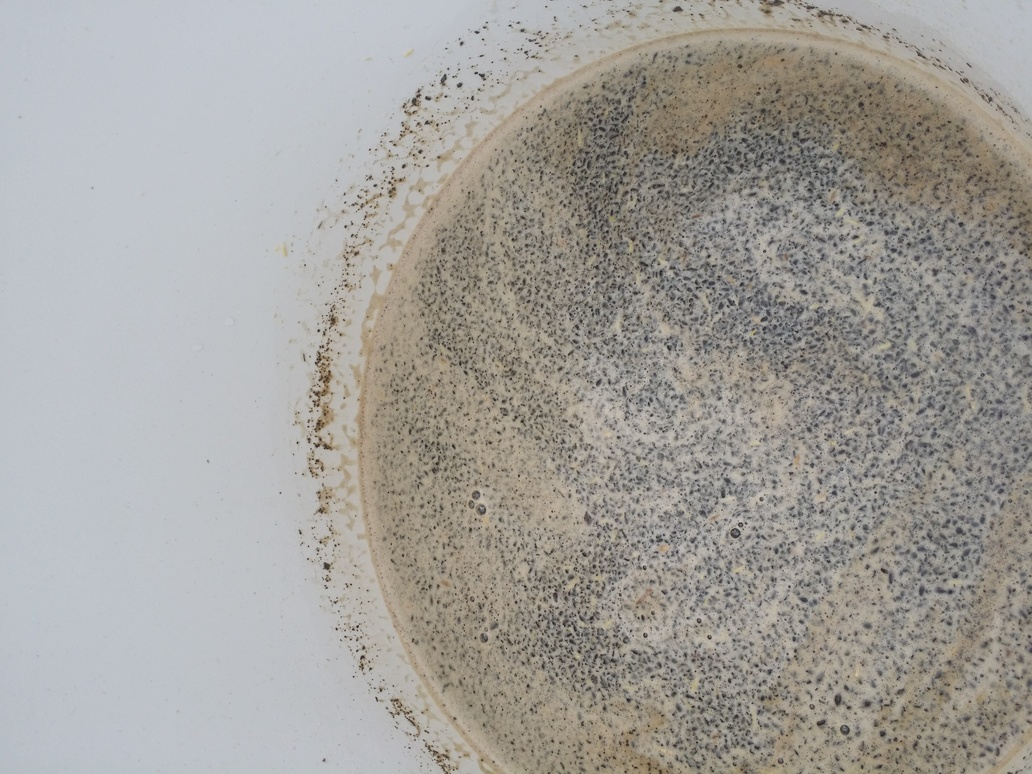
\includegraphics[width=0.5\textwidth]{IMG_20180520_084614_reduced}
  \caption{Mash}\label{fig:mash}
\end{figure}

\FloatBarrier{}
%------------------------------------------------------------------------------
\newentry[Cleaning]{0850 Cleaning}\FloatBarrier{}

Sanitize the primary firmentation bucket, tools and air-lock.  With the sanitizing compound in Figure~\ref{fig:sanitizer}, no rinse in plain water is required to remove the sanitizer.

\begin{figure}[H]
\begin{minipage}{0.45\textwidth}
  \centering
  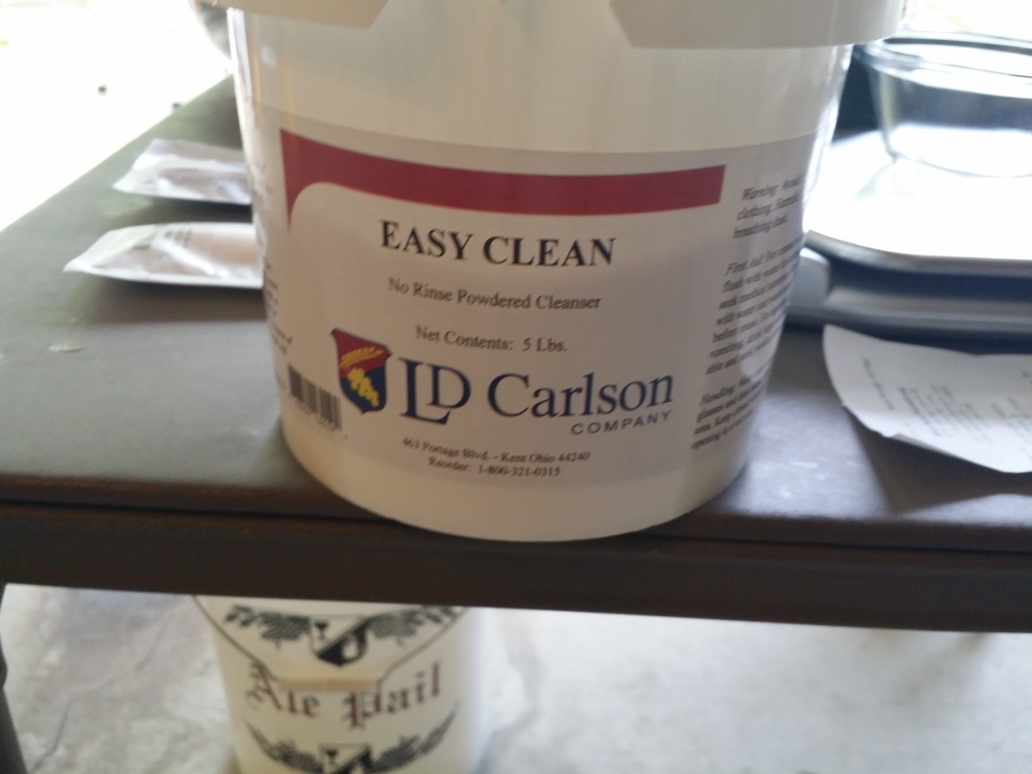
\includegraphics[width=\textwidth]{IMG_20180520_093004_reduced}
  \caption{No rinse sanitizer}\label{fig:sanitizer}
\end{minipage}\hfill
\begin{minipage}{0.45\textwidth}
  \centering
  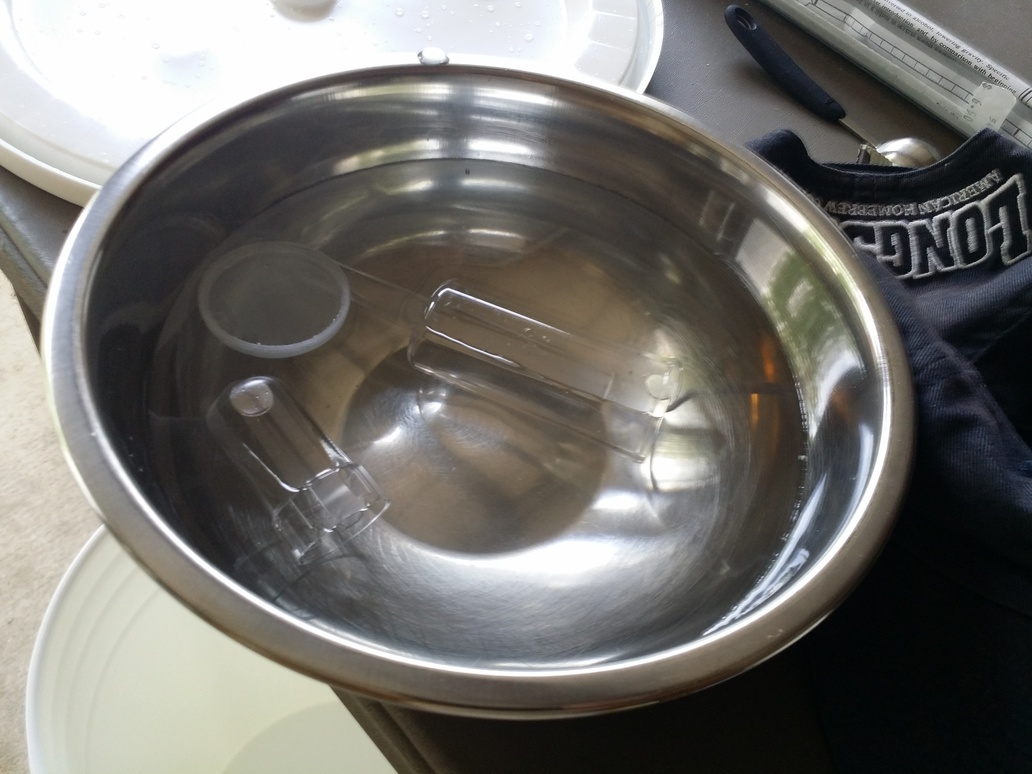
\includegraphics[width=\textwidth]{IMG_20180520_093016_reduced}
  \caption{Air-Lock Sanitizing}\label{fig:airlock}
\end{minipage}
\end{figure}

\FloatBarrier{}
%------------------------------------------------------------------------------
\newentry[Sparging]{0955 Sparging}\FloatBarrier{}

When timer was done wort was drawn from igloo silcock into a temporary container and then poured back into the igloo through top until the wort coming out of the silcock no longer had little bits of grain, as shown in Figure~\ref{fig:rinse}.  This cycles the fluid and places the little bits on top of the grain pile so they will be filtered out during sparging.

Setup the hot water sprayer on top of the igloo, being fed from the top pot as shown in Figure~\ref{fig:sparging}, and slowly spray water while draining out bottom into lower pan, Figure~\ref{fig:transfer}.  Go slow, this should take an hour.  As it starts to fill start heating the lower container, it will need to get to a rolling boil.  Figure~\ref{fig:gravitydrain} shows the sparging by draining heated water from the top container into the lautering tun, and then the wort being drained from the lautering tun into the lower boil pot.

\begin{figure}[H]
\centering
\begin{subfigure}[b]{.245\textwidth}
  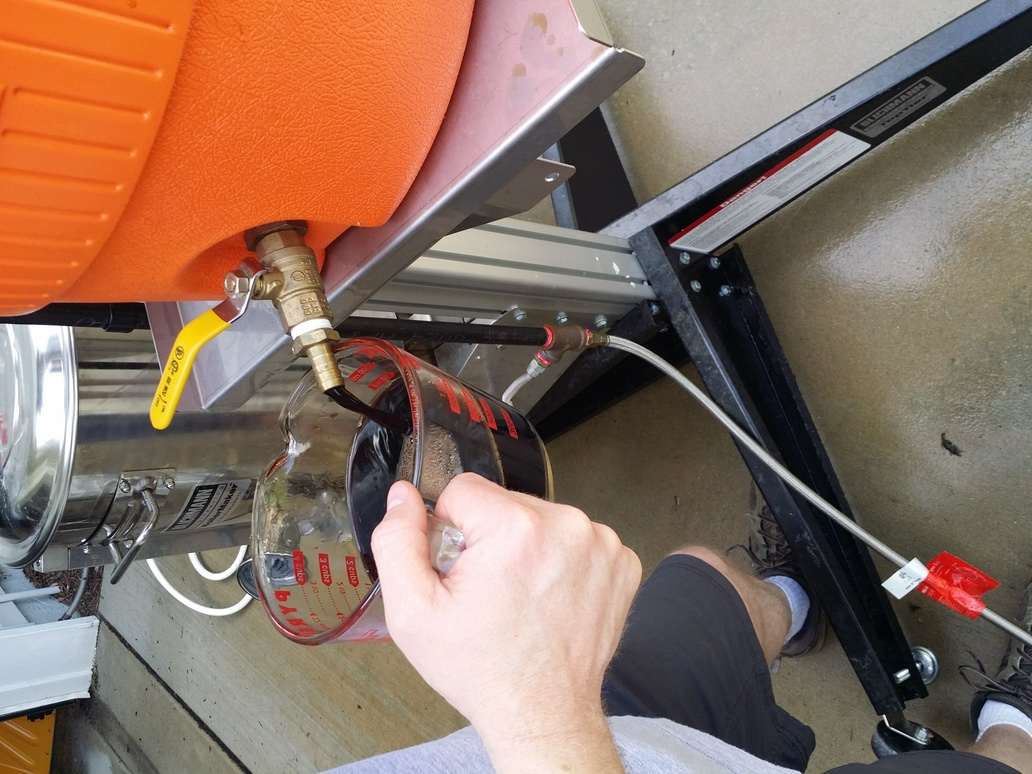
\includegraphics[angle=270,origin=c,width=\textwidth]{IMG_20180520_095406_reduced}
  \caption{Rinse}\label{fig:rinse}
\end{subfigure}
\begin{subfigure}[b]{.245\textwidth}
  \centering
  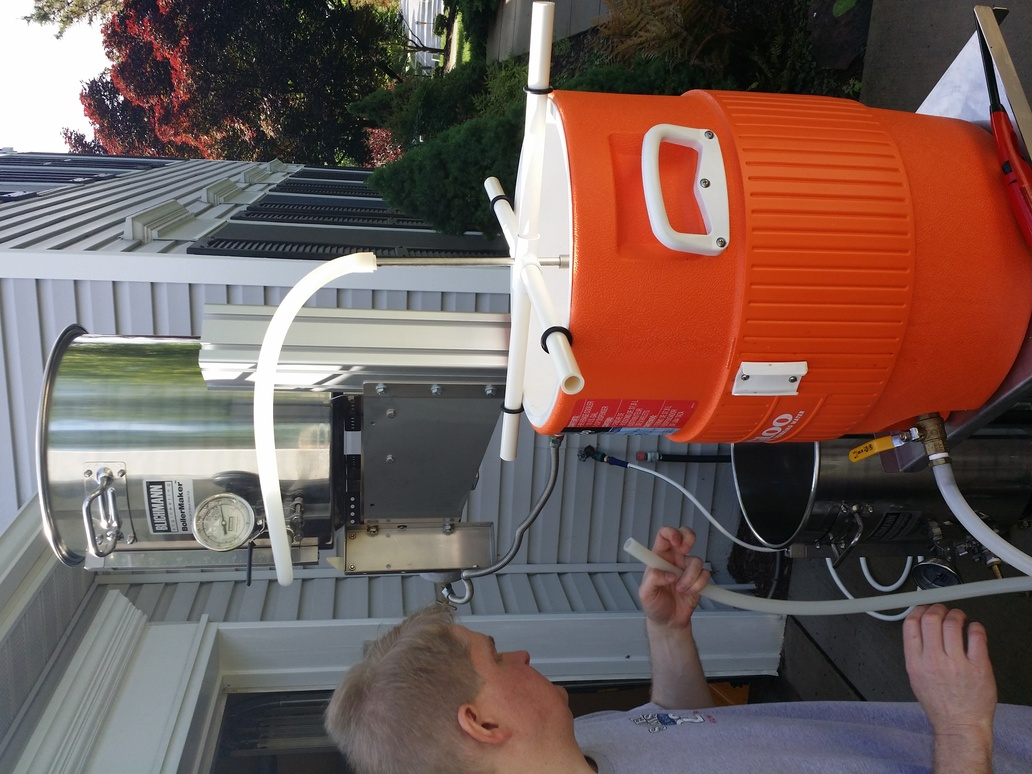
\includegraphics[angle=270,origin=c,width=\textwidth]{IMG_20180520_100013_reduced}
  \caption{Sparging}\label{fig:sparging}
\end{subfigure}
\begin{subfigure}[b]{.245\textwidth}
  \centering
  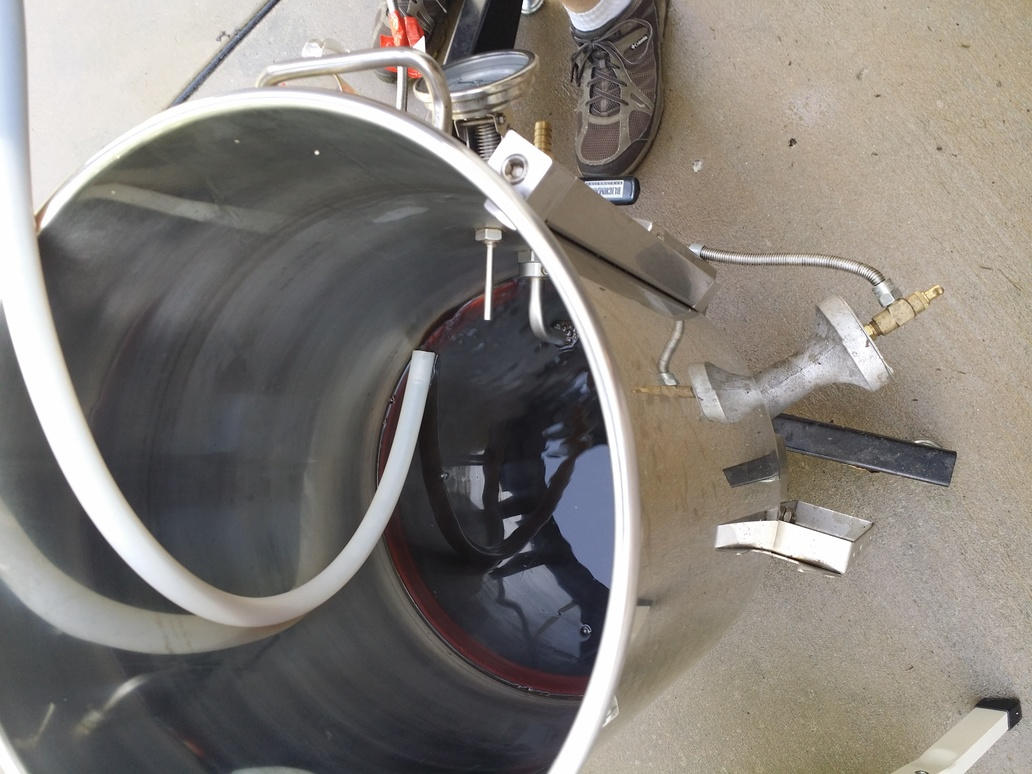
\includegraphics[angle=270,origin=c,width=\textwidth]{IMG_20180520_100206_reduced}
  \caption{Transfer for boil}\label{fig:transfer}
\end{subfigure}
\begin{subfigure}[b]{.245\textwidth}
  \centering
  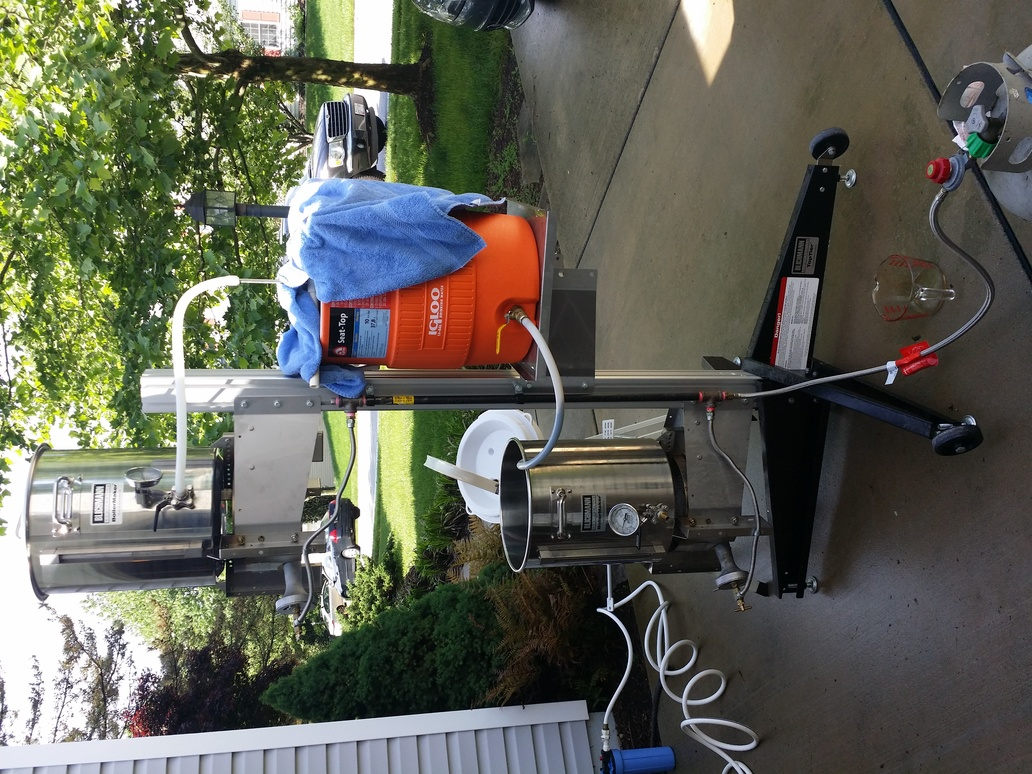
\includegraphics[angle=270,origin=c,width=\textwidth]{IMG_20180520_100432_reduced}
  \caption{Draining by gravity}\label{fig:gravitydrain}
\end{subfigure}
\caption{Sparging Process}\label{subfig:spargingprocess}
\end{figure}

\FloatBarrier{}
%------------------------------------------------------------------------------
\newentry[Boil Wort]{0955 Boil Wort}\FloatBarrier{}

Bring the wort to a rolling boil as shown in Figure~\ref{fig:boil}.  Measure out hops using a scale, and add to the boil according to recepie.

\begin{figure}[H]
  \centering
  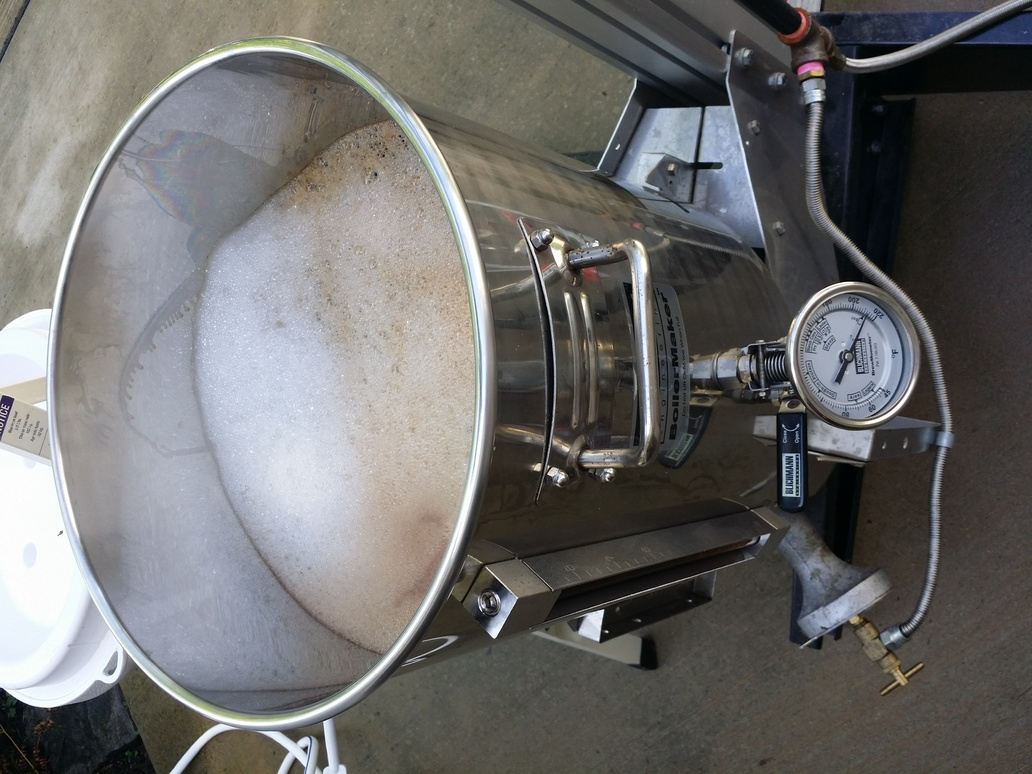
\includegraphics[angle=270,origin=c,width=0.95\textwidth]{IMG_20180520_110050_reduced}
  \caption{Boil}\label{fig:boil}
\end{figure}

\FloatBarrier{}
\clearpage
%------------------------------------------------------------------------------
\newentry[Cooling]{0955 Cooling}\FloatBarrier{}

Add the cooling coil at the end of boil but for several minutes while the boil to roll to sanitize the coil as shown in Figure~\ref{fig:cooling}.  The heat was turned off and coolling was begun by turning on the water to the cooling coil. The goal is to bring the temperature down to 70 degrees as quick as possible.

\begin{figure}[H]
  \centering
  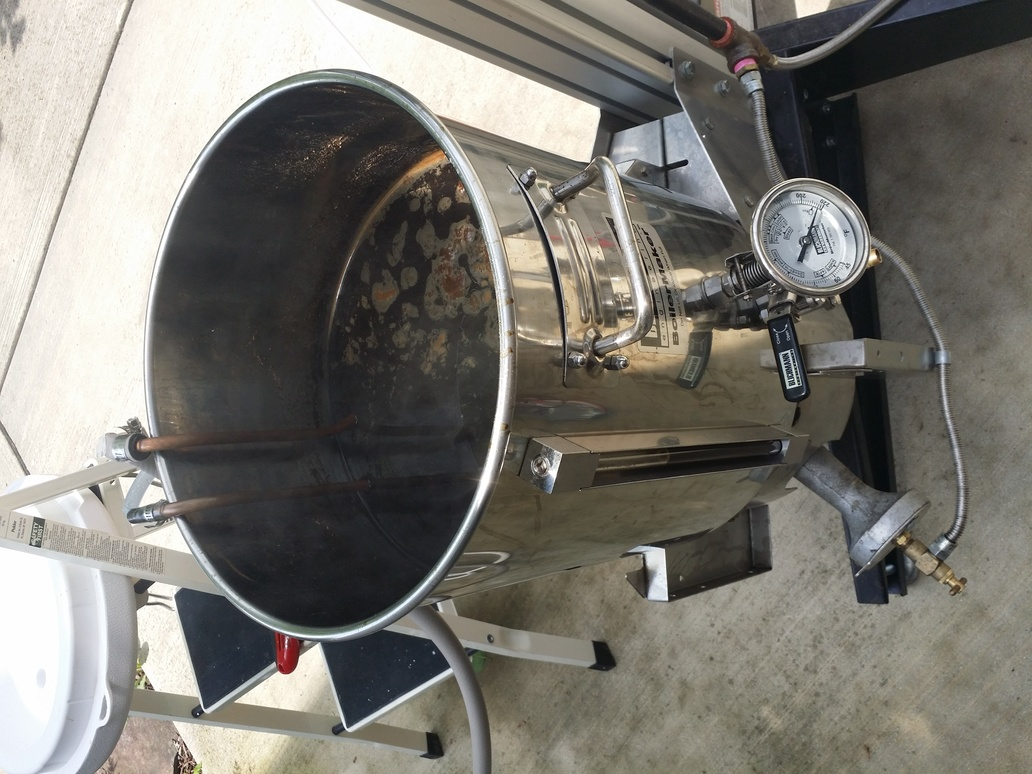
\includegraphics[angle=270,origin=c,width=0.95\textwidth]{IMG_20180520_123637_reduced}
  \caption{Cooling}\label{fig:cooling}
\end{figure}

\FloatBarrier{}
\clearpage
%------------------------------------------------------------------------------
\newentry[Transfer to Primary Firmentation Bucket]{0955 Transfer to Primary Firmentation Bucket}\FloatBarrier{}

Transfer to 5 gallon bucket as shown in Figure~\ref{fig:primary}, measure weight.

\begin{figure}[H]
  \centering
  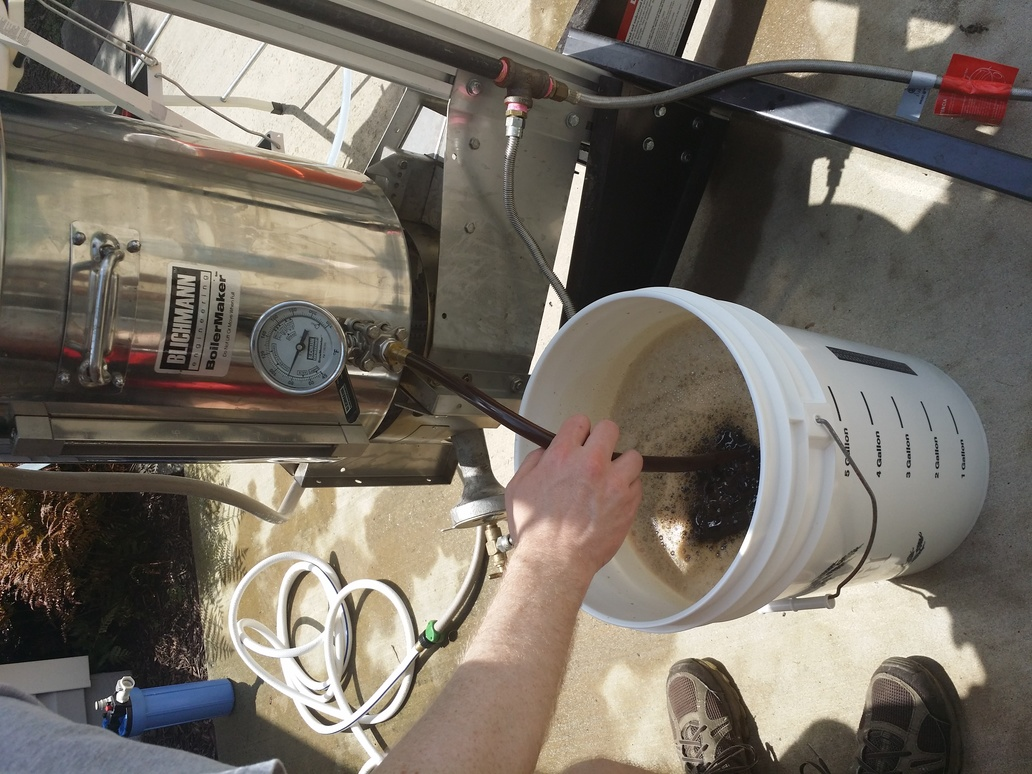
\includegraphics[angle=270,origin=c,width=\textwidth]{IMG_20180520_132938_reduced}
  \caption{Primary firmentation bucket}\label{fig:primary}
\end{figure}

\FloatBarrier{}
%------------------------------------------------------------------------------
\newentry[Aeration]{0955 Aeration}\FloatBarrier{}

Stir to aerate with oxygen for 10 to 15 minutes as shown in Figure~\ref{fig:aeration}. Watch the texture of the bubbles, as you are nearing finished, the bubbles will live longer.

\begin{figure}[H]
  \centering
  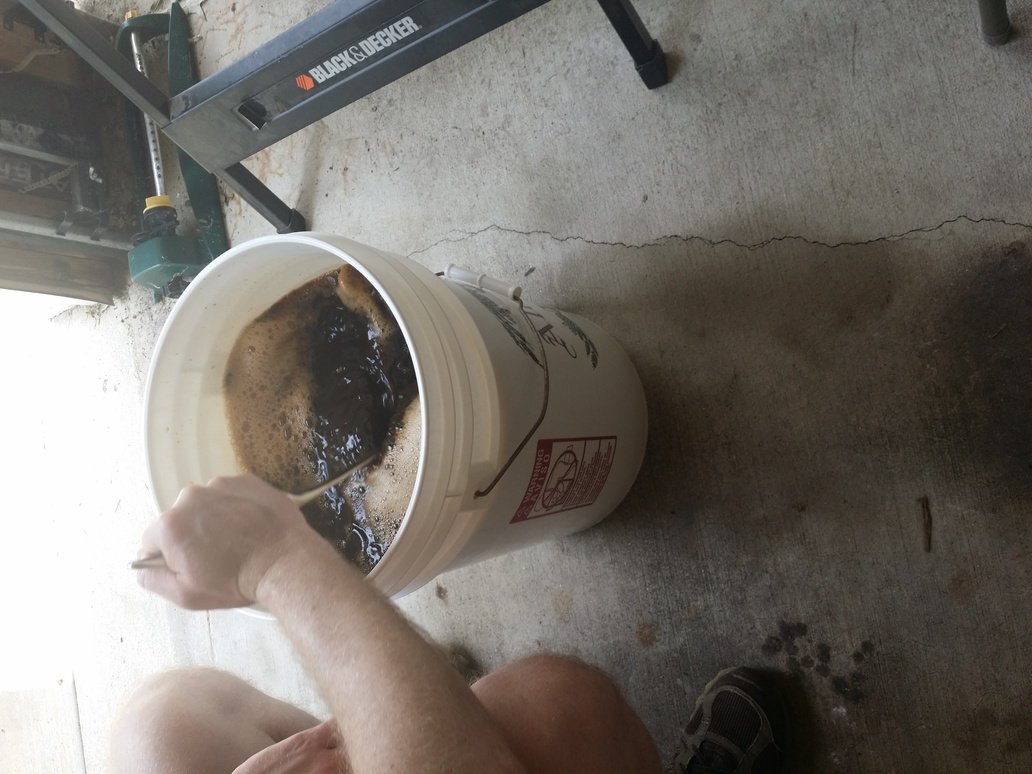
\includegraphics[angle=270,origin=c,width=\textwidth]{IMG_20180520_133334_reduced}
  \caption{Aeration}\label{fig:aeration}
\end{figure}

\FloatBarrier{}
%------------------------------------------------------------------------------
\newentry[Add Yeast]{0955 Add Yeast}\FloatBarrier{}

Sanitize the top edge of the bucket, sanitize yeast packet and scissors, open yeast and add to the bucket.  Stir in the yeast. Seal the bucket. Add one way valve for pressure escape and pour some sanitizer in the one way valve.

\begin{figure}[H]
  \centering
  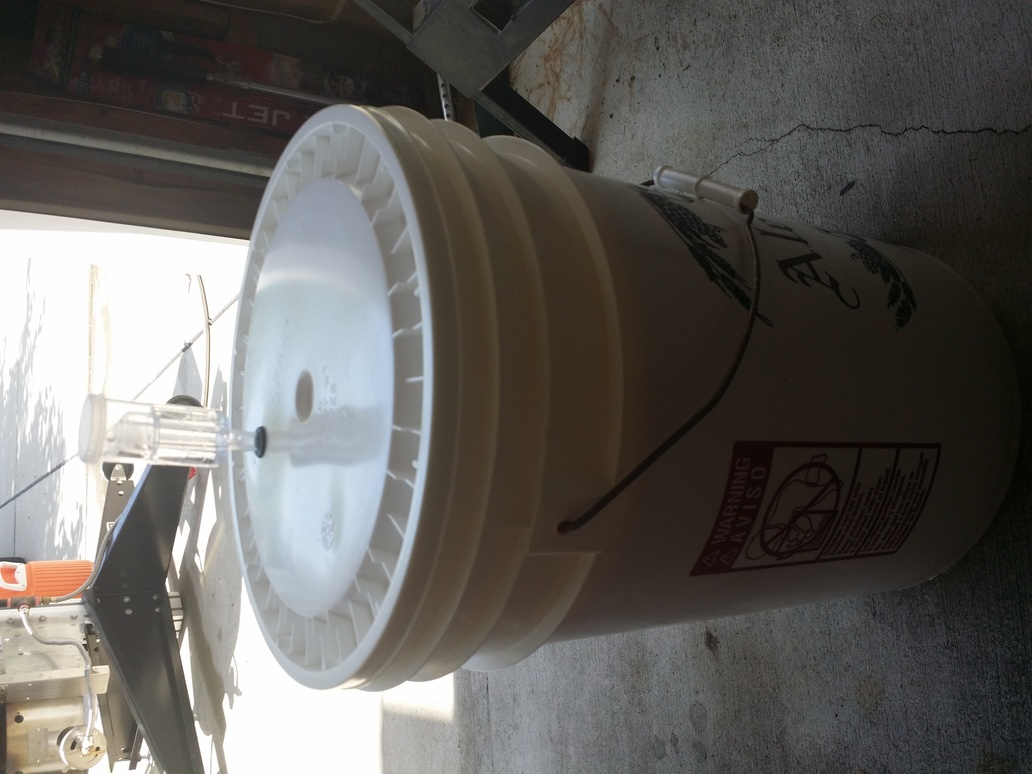
\includegraphics[angle=270,origin=c,width=0.95\textwidth]{IMG_20180520_134840_reduced}
  \caption{Sealed for primary firmentation}\label{fig:sealed}
\end{figure}

%------------------------------------------------------------------------------
%------------------------------------------------------------------------------
\newday{20180901}

\newentry[Homebrew System Planning]{0800 Homebrew System Planning}\FloatBarrier{}

After tasting the results of the~\hyperref[20180520]{May 20\textsuperscript{th}} brew, I have decided to start homebrewing myself.  The past several weeks I have been reading up on the processes and techniques and trying to sort out which of the many configurations for homebrewing will both work well for me, and provide an opportunity for fusion with other hobbies of mine, such as microcontroller programming, to be expanded later by automation.

\begin{table}[h!]
\centering
\begin{tabularx}{\textwidth}{clrcX}
    \toprule
    \multicolumn{1}{c}{\textbf{ID}} &\multicolumn{1}{c}{\textbf{Name}} & \multicolumn{1}{c}{\textbf{Price}} & \textbf{Quantity} & \multicolumn{1}{c}{\textbf{Link}} \\
    1 & Brewer's Edge Mash and Boil & \$299.99 & 1 & {\tiny\url{https://amazon.com/gp/product/B075NNZ3KT}} \\
    2 & Fermentation Lid & \$34.16 & 1 & {\tiny\url{https://amazon.com/gp/product/B077Y3RNK7}} \\
    3 & Sparge Water Heater & \$156.66 & 1 & {\tiny\url{https://amazon.com/gp/product/B01D05UHXQ}} \\
    4 & Chugger Pump & \$154.99 & 1 & {\tiny\url{https://amazon.com/gp/product/B01NCKU3ZC}} \\
    5 & Plate Chiller & \$89.99 & 1 & {\tiny\url{https://amazon.com/gp/product/B06Y44CS86}} \\
    6 & 5 Gallon Soda Keg & \$132.88 & 1 & {\tiny\url{https://amazon.com/gp/product/B00YREN4GM}} \\
    7 & Spoon & \$8.85 & 1 & {\tiny\url{https://amazon.com/gp/product/B001D6KF8M}} \\
    8 & Fermentation Bucket & \$36.73 & 1 & {\tiny\url{https://amazon.com/gp/product/B072B9X98X}} \\
    9 & Airlock & \$3.00 & 1 & {\tiny\url{https://amazon.com/gp/product/B000E60G2W}} \\
    10 & Ball Valve & \$22.90 & 1 & {\tiny\url{https://amazon.com/gp/product/B071GKPB6B}} \\
    11 & Wort Aerator & \$6.48 & 1 & {\tiny\url{https://amazon.com/gp/product/B00ODSS5J8}} \\
    12 & 3-Way Ball Valve & \$25.89 & 1 & {\tiny\url{https://amazon.com/gp/product/B07G72DFVQ}} \\
    13 & Male Hose Barb & \$8.50 & 1 & {\tiny\url{https://amazon.com/gp/product/B075VF861W}} \\
    14 & Female Hose Barb & \$7.25 & 1 & {\tiny\url{https://amazon.com/gp/product/B0064OJDUO}} \\
    15 & \#10 Rubber Stopper & \$4.95 & 1 & {\tiny\url{https://amazon.com/gp/product/B0057JB9XG}} \\
    17 & Silicone Tubing & \$19.55 & 1 & {\tiny\url{https://amazon.com/gp/product/B000FMWU38}} \\
    \bottomrule
\end{tabularx}
\caption{Parts List}\label{tab:partslist}
\end{table}

\tikzset{
block/.style = {draw, fill=white, rectangle, minimum height=3em, minimum width=3em},
tmp/.style  = {coordinate}, 
sum/.style= {draw, fill=white, circle, node distance=1cm},
input/.style = {coordinate},
output/.style= {coordinate},
pinstyle/.style = {pin edge={to-,thin,black}},
number/.style = {anchor=west,shape=circle,draw,inner sep=2pt}
}
\begin{figure}[H]
\centering
\begin{tikzpicture}[auto, node distance=2cm,>=latex']
    % Nodes
    \node (mashandboil) {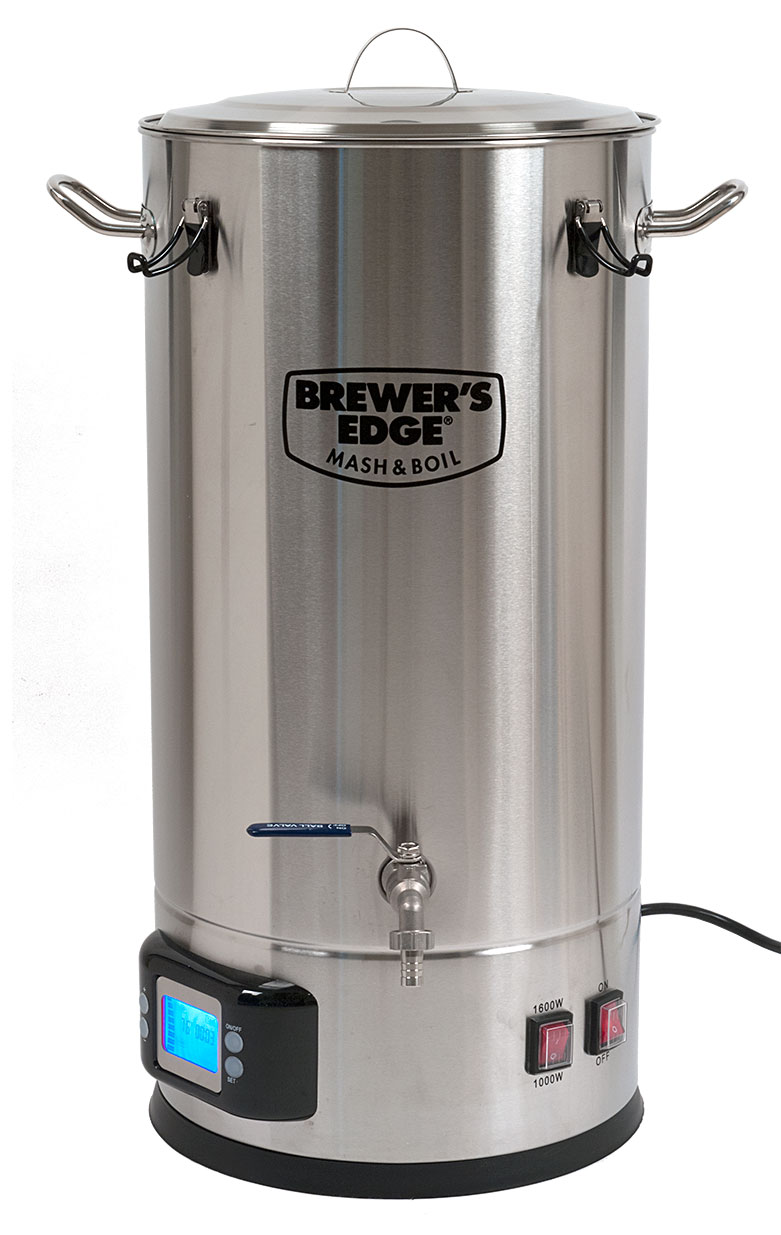
\includegraphics[width=1in]{mashandboil}};
    \node [left of=mashandboil, node distance=1in] (spargewater) {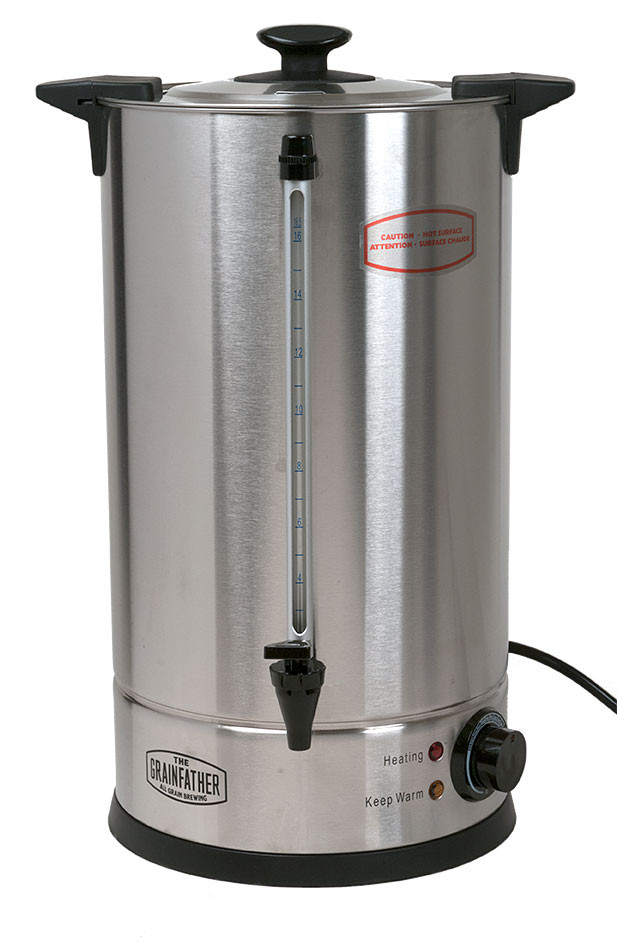
\includegraphics[width=1in]{spargewater}};
    \node [sum,below of=spargewater,node distance=1in] (swout) {};
    \node [sum,above of=mashandboil,node distance=1in] (mbin) {};
    \node [sum,below of=mashandboil,node distance=1in] (mbout) {};
    \node [right of=mbout] (chugger) {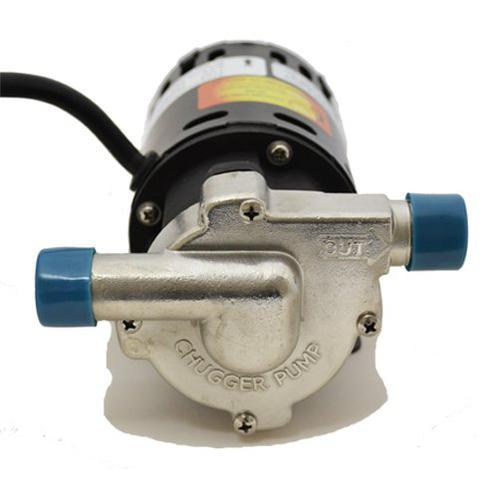
\includegraphics[width=0.5in]{chugger}};
    \node [spdt,above of=chugger,rotate=90] (switch1) {};
    \node [right of=switch1,yshift=0.6cm] (platechiller) {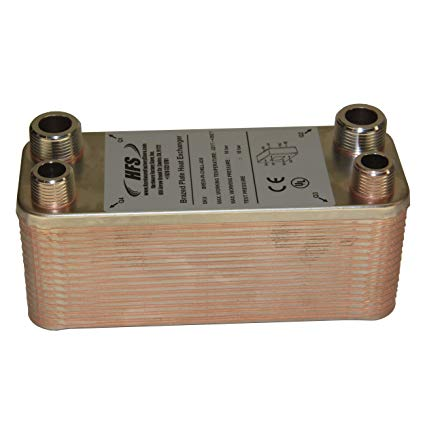
\includegraphics[width=0.5in]{platechiller}};
    \node [above of=platechiller] (tapwater) {Tap Water};
    \node [below of=platechiller] (drain) {Drain};
    \node [output,right of=platechiller] (pcout) {};
    
    % Lines
    \draw (mashandboil) -- (mbin);
    \draw (mashandboil) -- (mbout);
    \draw (spargewater) -- (swout);
    \draw (swout) -- (mbout);
    \draw (mbout) -- (chugger);
    \draw (chugger) -- (switch1.in);
    \draw (switch1.out 1) |- (mbin);
    \draw (switch1.out 2) -| (platechiller.west);
    \draw (platechiller) -- (pcout);
    \draw (platechiller) -- (tapwater);
    \draw (platechiller) -- (drain);
    \draw (pcout) |- (mbin);

    % Annotations
    \node [number] (1)  at (-1.45, 0.3) {1};
    \node [number] (3)  at (-4.0,  0.3) {3};
    \node [number] (4)  at ( 2.3, -3.1) {4};
    \node [number] (5)  at ( 3.1,  0.9) {5};
    \node [number] (10) at (-3.3, -3.0) {10};
    \node [number] (11) at (-1.0,  2.6) {11};
    \node [number] (12) at ( 1.9,  0.5) {12};
\end{tikzpicture}
\caption{Proposed Homebrew Configuration}\label{fig:config}
\end{figure}
\clearpage

The following is a proposed schedule for brew day using the configuration in Figure~\ref{fig:config}.

\begin{enumerate}
    \item Pour a beer.
    \item Add filtered water to sparge water heater and mash tun.
    \item Set mash tun to heat water to strike water temperature.
    \item Set sparge water heater to boil.
    \item Wait for strike water to come to temperature.
    \item Set flow control valve to bypass plate chiller.
    \item Mash in grain ingredients.
    \item Set timer.
    \item Start pump, and circulate at a slow rate into the top of the grain bed.
    \item Clean primary firmentation bucket, airlock, spoon, scissors, yeast package.
    \item Wait until timer is ended.
    \item Lift the grain tube to upper position.
    \item Close the valve on the mash tun, and open the sparge water valve, slowly sparging with  calculated needed water.
    \item Close the valve on the sparge water heater, remove the grain tube and place in primary firmentation bucket until ready to clean.
    \item Set mash tun to boil temperature.
    \item Add hops as instructed in the recipie.
    \item Clean grain tube.
    \item Set flow control valve to inline plate chiller.
    \item At five minutes left in the boil, leave the tap water valve closed, and open the valve on the mash tun to circulate boiling wort through the plate chiller to sanitize.
    \item Turn off mash tun heating element.
    \item Turn on tap water.
    \item Continue chilling till desired temperature is reached.
    \item Set flow control valve to bypass plate chiller, turn off tap water.
    \item Add yeast.
    \item Let pump circulate to aerate the wort and stir in yeast.
    \item Stop pump.
    \item Move wort aerator to primary firmentation bucket.
    \item Start pump and transfer wort from mash tun to primary firmentation bucket.
    \item Add airlock to primary firmentation bucket.
    \item Remove wort aerator from hose and place hose in drain.
    \item Set flow control valve to inline plate chiller.
    \item Open sparge water heater valve and drain remaining hot water through the plate chiller and into the drain.
    \item Turn off pump.
    \item Disconnect line from sparge water heater and re-connect to compressed air line.
    \item Open compressed air line just enough to purge water from lines, pump, and plate chiller.
    \item Pour another beer.
    \item Clean mash tun.
\end{enumerate}

The plan is to force carbonate in cornelius kegs.
%------------------------------------------------------------------------------
\newday{20180920}

\begin{figure}[H]
  \centering
  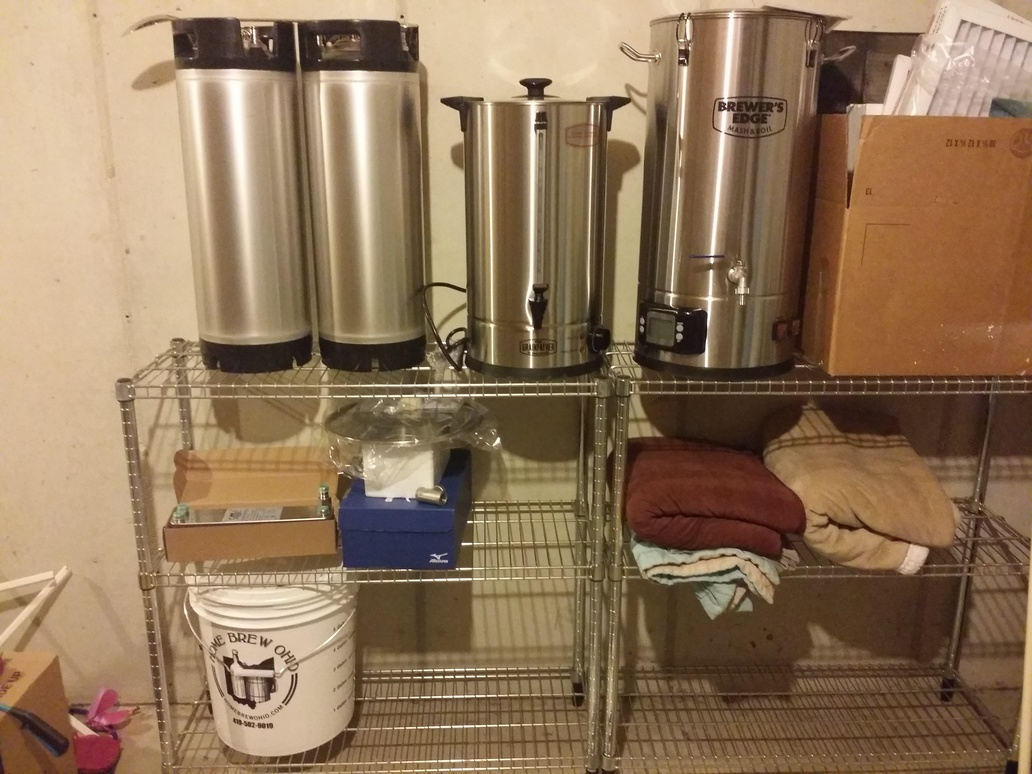
\includegraphics[angle=0,origin=c,width=\textwidth]{IMG_20180920_212437_reduced}
  \caption{Beginning Assembly of Brewing Equipment}\label{fig:temp}
\end{figure}

%------------------------------------------------------------------------------
\newday{20181014}

\newentry[Test Run]{0800 Test Run}\FloatBarrier{}


\begin{figure}[H]
  \centering
  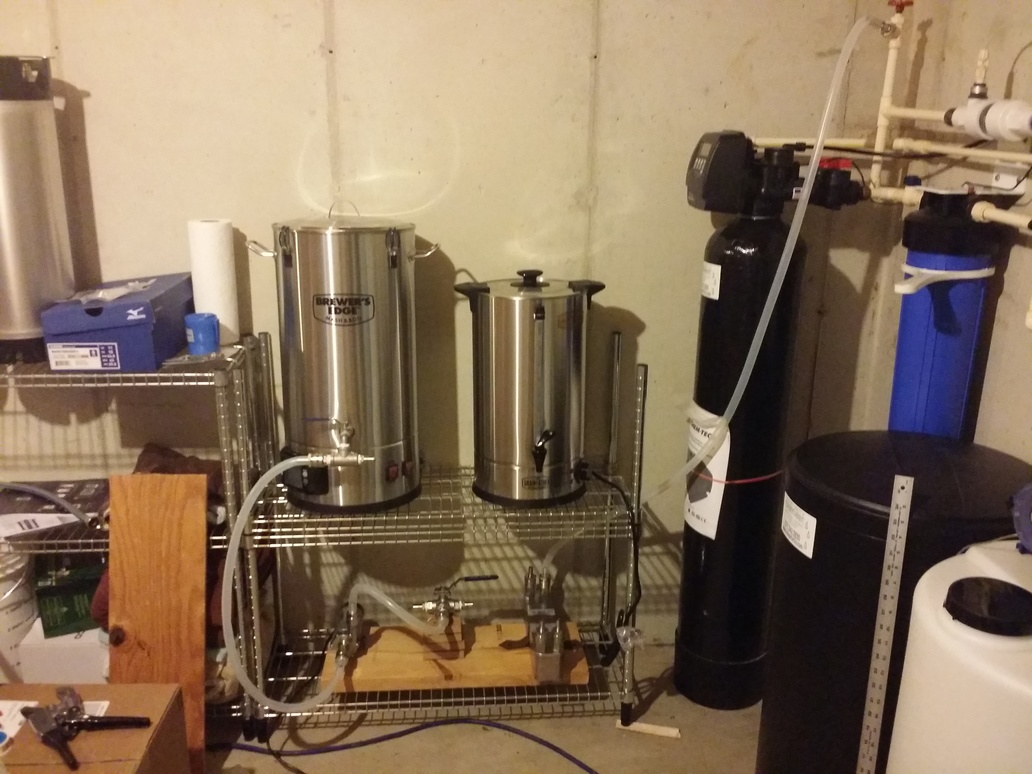
\includegraphics[angle=0,origin=c,width=\textwidth]{IMG_20181014_113442_reduced}
  \caption{Beginning Assembly of Brewing Equipment}\label{fig:temp}
\end{figure}

Running the system with just water today to evaluate the design and brew plan 
\begin{itemize}
    \item 
\end{itemize}

%------------------------------------------------------------------------------
\newday{20181028}

\newentry[Sparge Water Heater Modification]{0800 Sparge Water Heater Modification}\FloatBarrier{}

The sparge water heater has a plastic nozzle that will not attach to the quick hose disconnects easily.  I do not want to remove it, as it has an integrated water level indicator.  The temperature setting for heat is only in Celcius, and is not calibaratablle, so the plan is to install a good temperature probe next to the heat level dial, and a spicot with a fitting ready to receive a quick disconnect fitting on the other side of the existing spicot.

Using a step drill bit, shown below the thermometer in figure~\ref{fig:swm:drilled}, a \nicefrac{7}{8}\textsuperscript{th} inch hole was drilled for the ball valve (left of the existing spicot), and a \nicefrac{1}{2} inch hole was drilled for the temperature guage (right of the existing spicot).  I think a hole punch would have worked better as the step drill created a mess on the inside of shavings, and left the inside hole perimeter with large shards of razor sharp metal pressed in from the hole.  Instructions with some step drill bits recommend drilling from the other side to clean up the hole, but that was not possible with the locations of these holes inside the container.  Instead the holes were cleaned up by turning the step drill bit by hand on the inside, and by using files.  The resulting hole was not as clean as I would have liked it to be, or precise, even though figure~\ref{fig:swm:drilled} looks pretty good, it was not possible to take a picture from the inside with any clarity.  Once the fittings were installed as shown in figure~\ref{fig:swm:installed}, there were no leaks, so the process worked well enough.  As shown installed in figure~\ref{fig:swm:drilled}, a quick connect addapter was placed on the ball valve.

\begin{figure}[H]
  \centering
  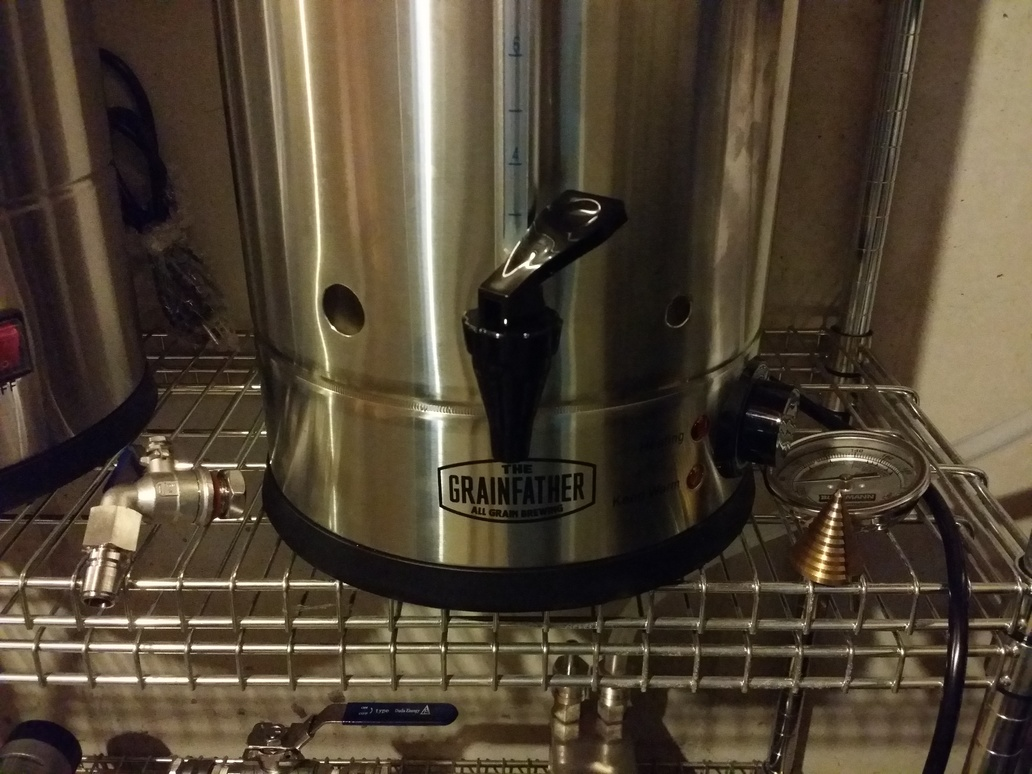
\includegraphics[angle=0,origin=c,width=\textwidth]{IMG_20181028_135028_reduced}
  \caption{Drilling Holes for Sparge Water Heater Modification}\label{fig:swm:drilled}
\end{figure}

\newentry[Test Run]{0800 Test Run}\FloatBarrier{}

\begin{figure}[H]
  \centering
  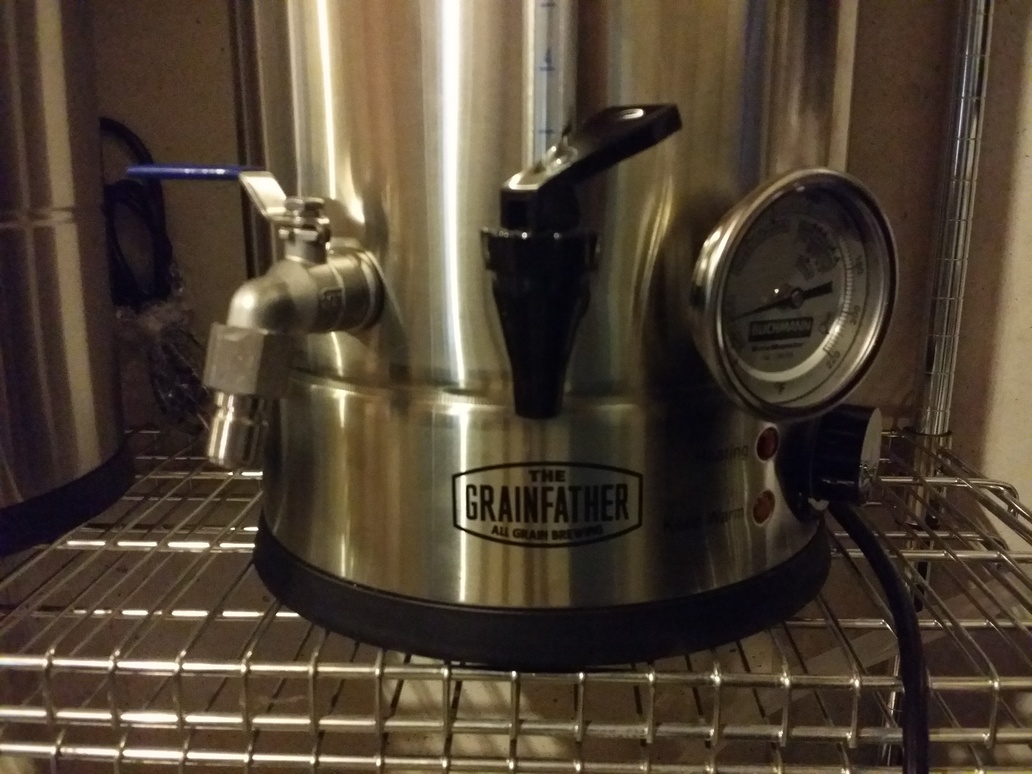
\includegraphics[angle=0,origin=c,width=\textwidth]{IMG_20181028_141228_reduced}
  \caption{Sparge Water Modifications Installed}\label{fig:swm:installed}
\end{figure}

%------------------------------------------------------------------------------
\newday{20181124}

\newentry[Homebrew Re-Design]{0800 Homebrew Re-Design}\FloatBarrier{}

After tasting the results of the~\hyperref[20180520]{May 20\textsuperscript{th}} brew, I have decided to start homebrewing myself.  The past several weeks I have been reading up on the processes and techniques and trying to sort out which of the many configurations for homebrewing will both work well for me, and provide an opportunity for fusion with other hobbies of mine, such as microcontroller programming, to be expanded later by automation.

\begin{table}[h!]
\centering
\begin{tabularx}{\textwidth}{clrcX}
    \toprule
    \multicolumn{1}{c}{\textbf{ID}} &\multicolumn{1}{c}{\textbf{Name}} & \multicolumn{1}{c}{\textbf{Price}} & \textbf{Quantity} & \multicolumn{1}{c}{\textbf{Link}} \\
    1 & Brewer's Edge Mash and Boil & \$299.99 & 1 & {\tiny\url{https://amazon.com/gp/product/B075NNZ3KT}} \\
    2 & Fermentation Lid & \$34.16 & 1 & {\tiny\url{https://amazon.com/gp/product/B077Y3RNK7}} \\
    3 & Sparge Water Heater & \$156.66 & 1 & {\tiny\url{https://amazon.com/gp/product/B01D05UHXQ}} \\
    4 & Chugger Pump & \$154.99 & 1 & {\tiny\url{https://amazon.com/gp/product/B01NCKU3ZC}} \\
    5 & Plate Chiller & \$89.99 & 1 & {\tiny\url{https://amazon.com/gp/product/B06Y44CS86}} \\
    6 & 5 Gallon Soda Keg & \$132.88 & 1 & {\tiny\url{https://amazon.com/gp/product/B00YREN4GM}} \\
    7 & Spoon & \$8.85 & 1 & {\tiny\url{https://amazon.com/gp/product/B001D6KF8M}} \\
    8 & Fermentation Bucket & \$36.73 & 1 & {\tiny\url{https://amazon.com/gp/product/B072B9X98X}} \\
    9 & Airlock & \$3.00 & 1 & {\tiny\url{https://amazon.com/gp/product/B000E60G2W}} \\
    10 & Ball Valve & \$22.90 & 1 & {\tiny\url{https://amazon.com/gp/product/B071GKPB6B}} \\
    11 & Wort Aerator & \$6.48 & 1 & {\tiny\url{https://amazon.com/gp/product/B00ODSS5J8}} \\
    12 & 3-Way Ball Valve & \$25.89 & 1 & {\tiny\url{https://amazon.com/gp/product/B07G72DFVQ}} \\
    13 & Male Hose Barb & \$8.50 & 1 & {\tiny\url{https://amazon.com/gp/product/B075VF861W}} \\
    14 & Female Hose Barb & \$7.25 & 1 & {\tiny\url{https://amazon.com/gp/product/B0064OJDUO}} \\
    15 & \#10 Rubber Stopper & \$4.95 & 1 & {\tiny\url{https://amazon.com/gp/product/B0057JB9XG}} \\
    17 & Silicone Tubing & \$19.55 & 1 & {\tiny\url{https://amazon.com/gp/product/B000FMWU38}} \\
    \bottomrule
\end{tabularx}
\caption{Parts List}\label{tab:partslist}
\end{table}

\tikzset{
block/.style = {draw, fill=white, rectangle, minimum height=3em, minimum width=3em},
tmp/.style  = {coordinate}, 
sum/.style= {draw, fill=white, circle, node distance=1cm},
input/.style = {coordinate},
output/.style= {coordinate},
pinstyle/.style = {pin edge={to-,thin,black}},
number/.style = {anchor=west,shape=circle,draw,inner sep=2pt}
}
\begin{figure}[H]
\centering
\begin{tikzpicture}[auto, node distance=2cm,>=latex']
    % Nodes
    \node (mashandboil) {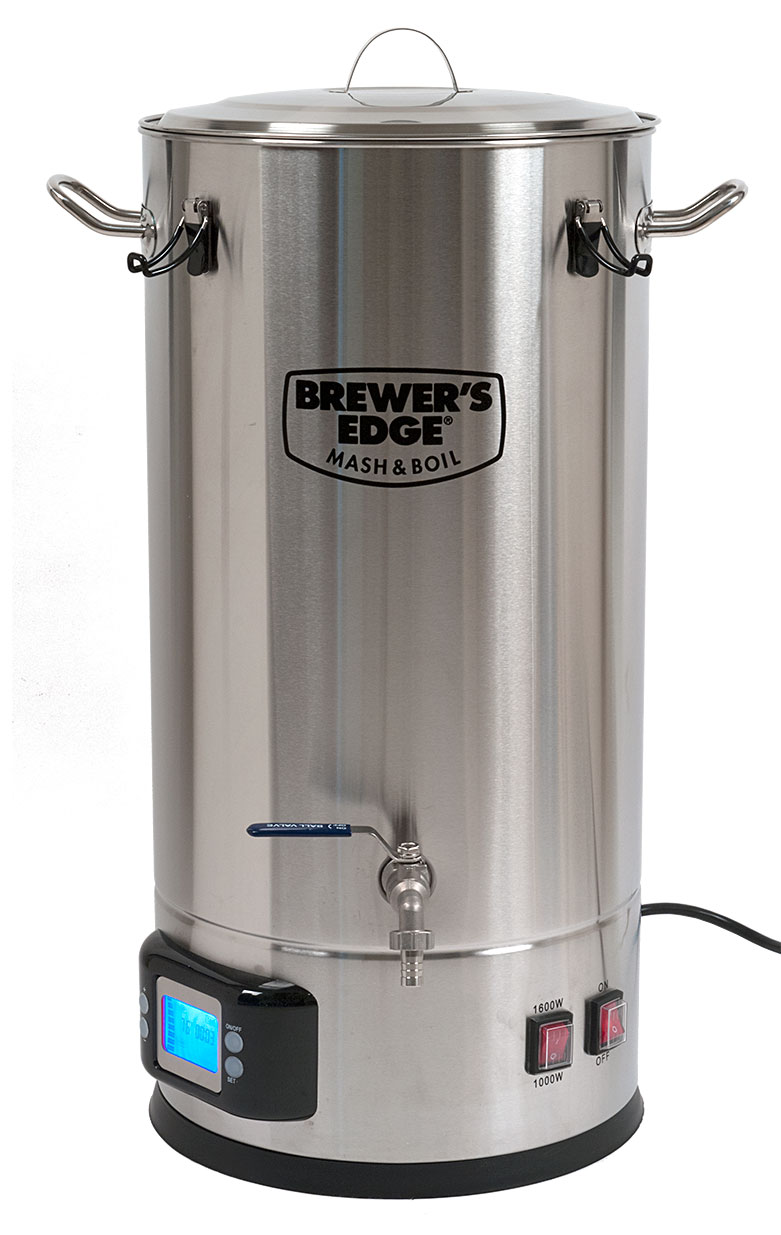
\includegraphics[width=1in]{mashandboil}};
    \node [left of=mashandboil, node distance=1in] (spargewater) {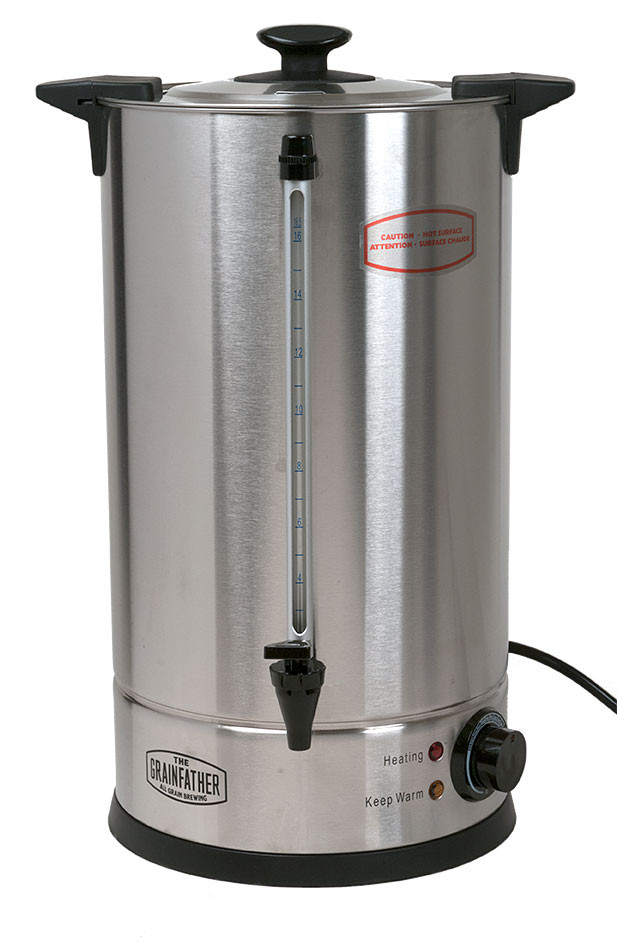
\includegraphics[width=1in]{spargewater}};
    \node [sum,below of=spargewater,node distance=1in] (swout) {};
    \node [sum,above of=mashandboil,node distance=1in] (mbin) {};
    \node [sum,below of=mashandboil,node distance=1in] (mbout) {};
    \node [right of=mbout] (chugger) {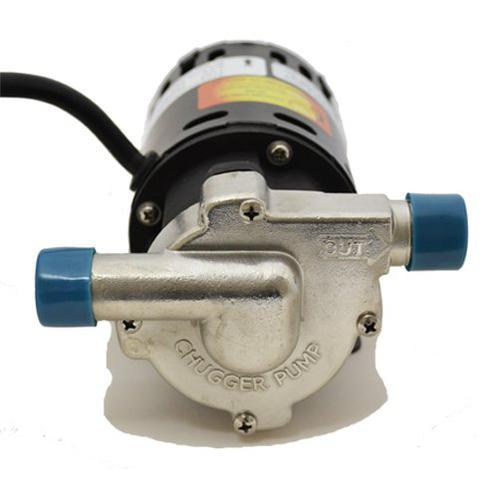
\includegraphics[width=0.5in]{chugger}};
    \node [spdt,above of=chugger,rotate=90] (switch1) {};
    \node [right of=switch1,yshift=0.6cm] (platechiller) {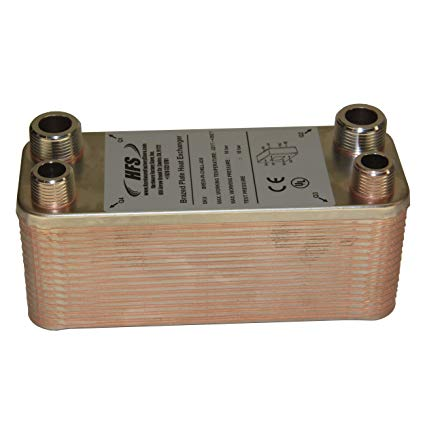
\includegraphics[width=0.5in]{platechiller}};
    \node [above of=platechiller] (tapwater) {Tap Water};
    \node [below of=platechiller] (drain) {Drain};
    \node [output,right of=platechiller] (pcout) {};
    
    % Lines
    \draw (mashandboil) -- (mbin);
    \draw (mashandboil) -- (mbout);
    \draw (spargewater) -- (swout);
    \draw (swout) -- (mbout);
    \draw (mbout) -- (chugger);
    \draw (chugger) -- (switch1.in);
    \draw (switch1.out 1) |- (mbin);
    \draw (switch1.out 2) -| (platechiller.west);
    \draw (platechiller) -- (pcout);
    \draw (platechiller) -- (tapwater);
    \draw (platechiller) -- (drain);
    \draw (pcout) |- (mbin);

    % Annotations
    \node [number] (1)  at (-1.45, 0.3) {1};
    \node [number] (3)  at (-4.0,  0.3) {3};
    \node [number] (4)  at ( 2.3, -3.1) {4};
    \node [number] (5)  at ( 3.1,  0.9) {5};
    \node [number] (10) at (-3.3, -3.0) {10};
    \node [number] (11) at (-1.0,  2.6) {11};
    \node [number] (12) at ( 1.9,  0.5) {12};
\end{tikzpicture}
\caption{Proposed Homebrew Configuration}\label{fig:config}
\end{figure}
\clearpage

Leading up to brew day, do the following\ldots
\begin{enumerate}
    \item Put .3 times the number of pounds in the 
\end{enumerate}
The following is a proposed schedule for brew day using the configuration in Figure~\ref{fig:config}.

\begin{enumerate}
    \item Pour a beer.
    \item Add filtered water to sparge water heater and mash tun.
    \item Set mash tun to heat water to strike water temperature.
    \item Set sparge water heater to boil.
    \item Wait for strike water to come to temperature.
    \item Set flow control valve to bypass plate chiller.
    \item Mash in grain ingredients.
    \item Set timer.
    \item Start pump, and circulate at a slow rate into the top of the grain bed.
    \item Clean primary firmentation bucket, airlock, spoon, scissors, yeast package.
    \item Wait until timer is ended.
    \item Lift the grain tube to upper position.
    \item Close the valve on the mash tun, and open the sparge water valve, slowly sparging with  calculated needed water.
    \item Close the valve on the sparge water heater, remove the grain tube and place in primary firmentation bucket until ready to clean.
    \item Set mash tun to boil temperature.
    \item Add hops as instructed in the recipie.
    \item Clean grain tube.
    \item Set flow control valve to inline plate chiller.
    \item At five minutes left in the boil, leave the tap water valve closed, and open the valve on the mash tun to circulate boiling wort through the plate chiller to sanitize.
    \item Turn off mash tun heating element.
    \item Turn on tap water.
    \item Continue chilling till desired temperature is reached.
    \item Set flow control valve to bypass plate chiller, turn off tap water.
    \item Add yeast.
    \item Let pump circulate to aerate the wort and stir in yeast.
    \item Stop pump.
    \item Move wort aerator to primary firmentation bucket.
    \item Start pump and transfer wort from mash tun to primary firmentation bucket.
    \item Add airlock to primary firmentation bucket.
    \item Remove wort aerator from hose and place hose in drain.
    \item Set flow control valve to inline plate chiller.
    \item Open sparge water heater valve and drain remaining hot water through the plate chiller and into the drain.
    \item Turn off pump.
    \item Disconnect line from sparge water heater and re-connect to compressed air line.
    \item Open compressed air line just enough to purge water from lines, pump, and plate chiller.
    \item Pour another beer.
    \item Clean mash tun.
\end{enumerate}

The plan is to force carbonate in cornelius kegs.
%------------------------------------------------------------------------------
\newday{20181217}

\newentry[Reverse Osmosis Water Collection]{1800 Reverse Osmosis Water Collection}\FloatBarrier{}
In preparation for this Friday's brew day, I will be collecting and storing reverse osmosis filtered water from my kitchen sink system.  The process to filter this water is slow, so each evening I will transfer 1-2 gallons from the filter reservoir to the 5 gallon corny kegs.  On brew day the water in the korny kegs will be transferred to the sparge water heater and mash tun.

%------------------------------------------------------------------------------
\newday{20181220}

\newentry[Grain and Supplies Purchase]{1400 Grain and Supplies Purchase}\FloatBarrier{}
Met with Damon at the Maryland Homebrewers store to purchase grain and supplies.

%------------------------------------------------------------------------------
\newday{20181221}

\newentry[Brew Day]{1000 Brew Day}\FloatBarrier{}
